\chapter{Коррекция и синтез расчетных динамических моделей конструкций}

Расчетные динамические модели разрабатываются на этапе проектирования ЛА. Они используются в оценках эксплуатационной нагруженности, обеспечении прочности, управляемости и аэроупругой устойчивости ЛА. По завершению расчетного этапа изготавливается ДПМ ЛА и проблема аэроупругой устойчивости решается экспериментально \cite{lib:modelUpdating:Karklje:GVT, lib:modelUpdating:Karklje:force}. Затем строится опытное изделие, а за ним и серийные. Расчетные динамические модели сопровождают экспериментальные исследования, опытную и серийную эксплуатацию ЛА. При этом расчетные модели корректируются по результатам наземных модальных испытаний, которым подвергаются ДПМ, опытные и выборочно серийные ЛА \cite{lib:modelUpdating:Karklje:GVT, lib:modelUpdating:Karklje:force, lib:modelUpdating:Heilen, lib:modelUpdating:Berns:monophase, lib:modelUpdating:Boswald, lib:modelUpdating:Brillhart, lib:modelUpdating:Peres, lib:modelUpdating:Peter, lib:modelUpdating:Pickrel, lib:modelUpdating:Baruch}.

Важно отметить, что расчетной моделью ЛА является модель свободной динамической системы. В то же время для модальных испытаний авиационная техника либо устанавливается на шасси, либо помещается на специальную систему упругого вывешивания, а космические конструкции~---~на систему обезвешивания. Системы упругого вывешивания и обезвешивания, влияние которых на свободную конструкцию строго регламентировано \cite{lib:modelUpdating:Berns:support}, являются сложными и дорогостоящими техническими сооружениями. Кроме того, известные методы коррекции математических моделей конструкций не предполагают использование моделей для граничных условий, отличных от тех, что были реализованы в эксперименте \cite{lib:modelUpdating:Mezhin, lib:modelUpdating:Kuznecov, lib:modelUpdating:Luo, lib:modelUpdating:Jang, lib:modelUpdating:Asgarieh, lib:modelUpdating:Sanayei, lib:modelUpdating:Wang}.

\section{Коррекция упругих характеристик} \label{struct:updating}

Пусть задана конечно-элементная модель исследуемого объекта в виде матриц жесткости $ \mat{K} $ и масс $ \mat{M} $, тогда собственные числа $ \lambda = 2 \pi \nu $ (где $ \nu $~---~частота собственных колебаний) и формы колебаний $ \mat{Y} $ определяются из решения обобщённой проблемы собственных значений:
\begin{equation}
	\rbrackets{\mat{K} - \lambda \mat{M}} \mat{Y} = 0
\end{equation}

Для изменения динамических свойств КЭ-модели, дополним её корректирующей моделью. Структура вводимой модели представлена внутренними и внешними корректирующими элементами. Первые определяют изменение характеристик самой модели, а вторые ответственны за коррекцию параметров внешних связей, накладываемых на модель. Корректирующие элементы строятся на узлах исходной модели. 

Обладая конструкторской документацией и результатами взвешивания конструкции, инерционные характеристики модели могут быть существенно уточнены. Изменение упругих характеристик модели не столь однозначно в силу совокупного объема факторов, обуславливающих погрешности моделирования: дискретизация модели, неточность задания упругих свойств материалов и граничных условий. Поэтому будем вносить изменения только в матрицу жесткости путем добавления к исходной матрице $ \mat{K} $ матрицы жесткости корректирующей КЭ-модели $ \Delta \mat{K} $, полагая матрицу масс определенной точно. При этом корректирующая матрица жесткости записывается в виде:
\begin{equation}
	\Delta \mat{K} = \Delta \internal{\mat{K}} + \Delta \external{\mat{K}}, \label{eq:stiffMatrixDecomposition}
\end{equation}
где $ \Delta \internal{\mat{K}} $ и $ \Delta \external{\mat{K}} $~---~матрицы жесткости внутренних и внешних корректирующих элементов.

Матрица жесткости внутреннего корректирующего элемента в общем случае имеет вид:
\begin{equation}
	\Delta \internal{\mat{K}}_j = \sum\limits_{p\,=\,1}^{q} \internal{c}_{j+p-1} \mat{G}_j^{(p)}, \ j = 1 \hdots e, \label{eq:updatingStiffnessMatrix}
\end{equation}
где $ \internal{c}_{j+p-1} $~---~неизвестная внутренняя корректирующая жесткость; $ q $~---~число внутренних корректирующих жесткостей, описывающих элемент; $ \mat{G}_j^{(p)} $~---~парциальная матрица жесткости внутреннего коррректирующего элемента; $ e $~---~число внутренних корректирующих элементов. Матрица~\eqref{eq:updatingStiffnessMatrix} симметричная, поэтому не нарушает симметрию матрицы жесткости корректируемой модели при суммировании с ней.

Число корректирующих жесткостей $ q $ зависит от числа физических параметров, которыми описывается добавляемый элемент. В случае, если динамические свойства модели существенно зависят от изгибных и крутильных жесткостей её балочных или оболочечных элементов, предлагается использовать корректирующую КЭ-модель из балочных элементов ($ q = 4 $). Тогда парциальные матрицы корректирующего элемента примут вид:
\begin{equation*}
	\mat{G}_j^{(1)} =
	\begin{pmatrix}
		\mat{D}_1 & 0 & -\mat{D}_1 & 0 \\
		0 & 0 & 0 & 0 \\
		-\mat{D}_1 & 0 & \mat{D}_1 & 0 \\
		0 & 0 & 0 & 0 \\
	\end{pmatrix},
	\mat{G}_j^{(2)} =
	\begin{pmatrix}
		6 \mat{D}_2 & 3 \ell \mat{D}_4 & -6 \mat{D}_2 & 3 \ell \mat{D}_4 \\
		3 \ell \trans{\mat{D}}_4 & 2 \ell ^ 2 \mat{D}_3 & -3 \ell \trans{\mat{D}}_4 & \ell ^ 2 \mat{D}_3 \\
		-6 \trans{\mat{D}}_2 & -3 \ell \mat{D}_4 & 6 \mat{D}_2 & -3 \ell \mat{D}_4 \\
		3 \ell \trans{\mat{D}}_4 & \ell ^ 2 \trans{\mat{D}}_3 & -3 \ell \trans{\mat{D}}_4 & 2 \ell ^ 2 \mat{D}_3
	\end{pmatrix},
\end{equation*}

\begin{equation*}
	\mat{G}_j^{(3)} =
	\begin{pmatrix}
		6 \mat{D}_3 & -3 \ell \trans{\mat{D}}_4 & -6 \mat{D}_3 & -3 \ell \trans{\mat{D}}_4 \\
		-3 \ell \mat{D}_4 & 2 \ell ^ 2 \mat{D}_2 & 3 \ell \mat{D}_4 & \ell ^ 2 \mat{D}_2 \\
		-6 \trans{\mat{D}}_3 & 3 \ell \trans{\mat{D}}_4 & 6 \mat{D}_3 & 3 \ell \trans{\mat{D}}_4 \\
		-3 \ell \mat{D}_4 & \ell ^ 2 \trans{\mat{D}}_2 & 3 \ell \mat{D}_4 & 2 \ell ^ 2 \mat{D}_2
	\end{pmatrix},
	\mat{G}_j^{(4)} =
	\begin{pmatrix}
		0 & 0 & 0 & 0 \\
		0 & \mat{D}_1 & 0 & -\mat{D}_1 \\
		0 & 0 & 0 & 0 \\
		0 & -\mat{D}_1 & 0 & \mat{D}_1 \\
	\end{pmatrix},
\end{equation*}
где $ \ell $~---~длина корректирующего балочного элемента; $ D_1, D_2, D_3, D_4 $~---~матрицы, состоящие из направляющих косинусов:
\begin{gather*}
	\mat{D}_k = 
	\begin{pmatrix}
		d_{k, 1}^2 & d_{k, 1} d_{k, 2} & d_{k, 1} d_{k, 3} \\
		d_{k, 2} d_{k, 1} & d_{k, 2} ^ 2 & d_{k, 2} d_{k, 3} \\
		d_{k, 3} d_{k, 1} & d_{k, 3} d_{k, 2} & d_{k, 3} ^ 2
	\end{pmatrix}, \ k = 1 \hdots 3, \\
	\mat{D}_4 = 
	\begin{pmatrix}
		d_{2, 1} d_{3, 1} & d_{2, 1} d_{3, 2} & d_{2, 1} d_{3, 3} \\
		d_{2, 2} d_{3, 1} & d_{2, 2} d_{3, 2} & d_{2, 2} d_{3, 3} \\
		d_{2, 3} d_{3, 1} & d_{2, 3} d_{3, 2} & d_{2, 3} d_{3, 3}
	\end{pmatrix}.
\end{gather*}

Для коррекции модели, составленной из объемных элементов, в качестве корректирующей КЭ-модели используется ферменная конструкция ($ q = 1 $). 

В качестве внешних корректирующих элементов предлагается использовать пружинные опоры, прикрепленные к неподвижному основанию. Тогда матрица $ \Delta \external{\mat{K}} $ равна:
\begin{equation}
	\Delta \external{\mat{K}} = \operatorname{diag} \cbrackets{\external{c}_1, \external{c}_2, \hdots, \external{c}_N},
\end{equation}
где $ N $~---~размерность КЭ-модели, $ \external{c} $~---~неизвестные внешние корректирующие жесткости. 

Заметим, что жесткости корректирующих элементов могут быть отрицательными для изменения упругости конструкции в сторону уменьшения. При этом жесткости каждого вводимого элемента являются параметрами коррекции, которые подлежат определению из решения задачи безусловной минимизации целевой функции. Полный вектор разыскиваемых параметров записывается по всем жесткостям внутренних и внешних корректирующих элементов: $ \mat{c} = \rbrackets{\internal{\mat{c}}, \external{\mat{c}}} $.

На рисунке \ref{fig:principalSchemeUpdating} приведена принципиальная схема, иллюстрирующая физическую сторону предлагаемого метода на примере простой модели летательного аппарата. В данном случае модель составлена из объемных и оболочечных элементов, поэтому для изменения её динамических свойств вводятся как балочные, так и ферменные корректирующие элементы. Кроме того, для описания модели упругого основания, вводятся пружинные элементы. Таким образом, корректирующая модель образует <<каркасную>> структуру над исходной моделью.

\begin{figure}[!htb]
	\centerfloat
	\begin{tikzpicture}[scale = 1]
		\pgfmathsetmacro{\nodeDist}{0.2}
		\pgfmathsetmacro{\shiftText}{0.0}
		% Исходная модель
		\node[inner sep = 0pt] (initial) at (0, 0) {\includegraphics[width = 0.4\textwidth]{simple-model-initial}};
		\node[inner sep = 0pt, below = \shiftText of initial.south] (textInitial) {Исходная модель};
		% Знак
		\node [below = \nodeDist of textInitial.south, color = blue] (sumSign) {\Huge \bfseries +};
		% Коррректирующие элементы
		\node[inner sep = 0pt, below = -\nodeDist of sumSign.south] (elements) {\includegraphics[width = 0.4\textwidth]{simple-model-elements}};
		\node[inner sep = 0pt, below = \shiftText of elements.south] (textElements) {Корректирующие элементы};
		% Скорректированная модель
		\draw [-{Latex[length = 4mm]}, color = red, ultra thick](sumSign.east) ++ (3, 0) --++ (1, 0) node [right] (updated) {\includegraphics[width = 0.5\textwidth]{simple-model-updated}};
		\node[inner sep = 0pt, below = \shiftText of updated.south] (textUpdated) {Скорректированная модель};
	\end{tikzpicture}
	\caption{Принципиальная схема коррекции} \label{fig:principalSchemeUpdating}
\end{figure}

Для автоматического формирования набора внутренних корректирующих элементов используется портрет матрицы жесткости корректируемой конструкции. Так, если в матрице линейные степени свободы двух узлов <<связаны>> между собой внедиагональными элементами, то добавляется корректирующий элемент между этими узлами. В общем случае число таких корректирующих элементов определяется количеством связей между узлами в матрице, но оно может быть уменьшено посредством выбора областей коррекции, например, элементов конструкции с наибольшей неопределенностью физических и геометрических характеристик. Кроме того, число независимых корректирующих жесткостей может быть уменьшено посредством введения зависимостей между элементами. Например, могут быть учтены геометрические особенности конструкции: наличие плоскостей симметрии и конструктивно идентичных элементов. Дополнительно могут быть назначены узлы для введения внешних корректирующих элементов, описывающих линейные и вращательные упругие связи. Кроме того, можно проводить поэтапную коррекцию, в ходе которой в качестве целевых принимаются различные группы частот.

В зависимости от геометрии модели и типов конечных элементов может получиться так, что при добавлении \eqref{eq:updatingStiffnessMatrix} к матрице жесткости исходной конструкции появятся новые ненулевые элементы (изменится портрет разреженной матрицы). Такая ситуация возникает, например, когда есть геометрическая симметрия относительно некоторого узла и в исходном портрете соответствующие элементы при ассемблировании матрицы жесткости в сумме дают ноль и не попадают в портрет. Поэтому перед началом процедуры коррекции портрет матрицы жесткости дополняется портретом корректирующей матрицы.

Рассмотрим алгоритм метода коррекции на примере одного целевого значения для упрощения индексных обозначений, а затем обобщим формулы для случая коррекции по нескольким значениям собственных частот. Пусть в результате коррекции необходимо достигнуть целевого значения $ \lambda ^ \ast $. Необходимо найти такую $ \Delta \mat{K} ^ \ast $, чтобы достигнуть значения $ \lambda ^ \ast $ при решении следующей обобщенной проблемы:
\begin{equation}
	\sbrackets{\rbrackets{\mat{K} + \Delta \mat{K} ^ \ast} - \lambda ^ \ast \mat{M}} \mat{Y} ^ \ast = 0
	\label{eq:targetEigProblem}
\end{equation}

Так как в \eqref{eq:targetEigProblem} собственный вектор $ \mat{Y} ^ \ast $ зависит от матрицы $ \Delta \mat{K} ^ \ast $, то использовать \eqref{eq:targetEigProblem} напрямую как нелинейное матричное уравнение для поиска корректирующих жесткостей слишком затратно с вычислительной точки зрения: придется многократно решать обобщенную проблему. Поэтому для поиска корректирующей матрицы $ \Delta \mat{K} ^ \ast $ предлагается следующий итерационный алгоритм.

Пусть решена обобщенная проблема для исходной модели
\begin{equation}
	\rbrackets{\mat{K} - \lambda ^ {(0)} \mat{M}} \mat{Y} ^ {(0)} = 0,
	\label{eq:initEigProblem}
\end{equation}
то есть найдены $ \lambda ^ {(0)} $ и $ \mat{Y} ^ {(0)} $. Здесь и далее верхний индекс в круглых скобках обозначает номер итерации. На первой итерации ищем такое $ \Delta \mat{K} ^ {(1)} $, чтобы удовлетворить следующему уравнению:
\begin{equation}
	\sbrackets{\rbrackets{\mat{K} + \Delta \mat{K} ^ {(1)}} - \lambda ^ \ast \mat{M}} \mat{Y} ^ {(0)} = 0.
	\label{eq:firstUpdatingIteration}
\end{equation}

Здесь необходимо отметить, что $ \Delta \mat{K} ^ {(1)} $ является функцией от корректирующих жесткостей $ c_1, c_2, \hdots, c_m $. 

Число корректирующих жесткостей $ m $ в общем случае равняется $ e + N $, а следовательно, больше числа уравнений в \eqref{eq:firstUpdatingIteration}. Поэтому для решения \eqref{eq:firstUpdatingIteration} необходимо устремить к нулю следующую скалярную величину (невязку):
\begin{equation}
	f ^ {(1)} = \trans{\rbrackets{\mat{Y} ^ {(0)}}} \sbrackets{\Delta \mat{K} ^ {(1)} - \Delta \lambda ^ {(1) \ast} \mat{M}} \mat{Y} ^ {(0)},
	\label{eq:firstResidualUpdating}
\end{equation}
где $ \Delta \lambda ^ {(1) \ast} = \lambda ^ \ast - \lambda ^ {(0)} $.

В результате минимизации невязки \eqref{eq:firstResidualUpdating} по корректирующим жесткостям получим $ \Delta \mat{K} ^ {(1)} $ и, решив новую обобщённую проблему
\begin{equation}
	\sbrackets{\rbrackets{\mat{K} + \Delta \mat{K} ^ {(1)}} - \lambda ^ {(1)} \mat{M}} \mat{Y} ^ {(1)} = 0,
\end{equation}
найдем $ \lambda ^ {(1)} $ и $ \mat{Y} ^ {(1)} $. Это первая итерация метода. Аналогично \eqref{eq:firstUpdatingIteration} составим следующее уравнение для поиска $ \Delta \mat{K} ^ {(2)} $:
\begin{equation}
	\sbrackets{\rbrackets{\mat{K} + \Delta \mat{K} ^ {(1)} + \Delta \mat{K} ^ {(2)}} - \lambda ^ \ast \mat{M}} \mat{Y} ^ {(1)} = 0,
	\label{eq:secondUpdatingIteration}
\end{equation}
представим $ \lambda ^ \ast = \rbrackets{\lambda ^ {(1)} + \Delta \lambda ^ {(2) \ast}} $, тогда \eqref{eq:secondUpdatingIteration} перепишется в следующем виде:
\begin{equation}
	\begin{matrix}
		\sbrackets{\rbrackets{\mat{K} + \Delta \mat{K} ^ {(1)} + \Delta \mat{K} ^ {(2)}} - \rbrackets{\lambda ^ {(1)} + \Delta \lambda ^ {(2) \ast}} \mat{M}} \mat{Y} ^ {(1)} = 0; \\
		\sbrackets{\Delta \mat{K} ^ {(2)} - \Delta \lambda ^ {(2) \ast} \mat{M}} \mat{Y} ^ {(1)} = 0,
	\end{matrix}
\end{equation}
где $ \Delta \lambda ^ {(2) \ast} = \lambda ^ \ast - \lambda ^ {(1)} $. Аналогично \eqref{eq:firstResidualUpdating} устремим к нулю невязку
\begin{equation}
	f ^ {(2)} = \trans{\rbrackets{\mat{Y} ^ {(1)}}} \sbrackets{\Delta \mat{K} ^ {(2)} - \Delta \lambda ^ {(2) \ast} \mat{M}} \mat{Y} ^ {(1)}.
\end{equation}

Это была вторая итерация метода коррекции. Обобщим формулы на случай нескольких целевых собственных значений. Пусть их число равно $ s $. Таким образом, на каждой итерации метода коррекции минимизируется следующая целевая функция:
\begin{gather}
	F ^ {(j + 1)}(c_1, c_2, \hdots, c_m) = \sum\limits_{i\,=\,1}^s w_i \sbrackets{f_i ^ {(j + 1)}} ^ 2 = \nonumber \\
	= \sum\limits_{i = 1} ^ s w_i \sbrackets{\trans{\rbrackets{\mat{Y}_i ^ {(j)}}} \Delta \mat{K} ^ {(j + 1)} \mat{Y}_i ^ {(j)} - \Delta \lambda_i ^ {(j + 1) \ast} \trans{\rbrackets{\mat{Y}_i ^ {(j)}}} \mat{M} \mat{Y}_i ^ {(j)}} \rightarrow \min,
	\label{eq:objFunUpdating}
\end{gather}
где $ j $~---~номер итерации, $ w_i $~---~весовой коэффициент $ i $-го тона.

Для минимизации \eqref{eq:objFunUpdating} используется метод сопряженных градиентов. С вычислительной точки зрения важно найти аналитические выражения для вектора-градиента целевой функции. Для этого найдем производные от целевой функции по неизвестным корректирующим жесткостям (здесь и далее опустим номер итерации в круглых скобках):
\begin{equation}
	\partDer{F}{c_p}{} = 2 \sum\limits_{i\,=\,1} ^ s w_i f_i \partDer{f_i}{c_p}{}, \ p = 1 \hdots m.
	\label{eq:derObjFunUpdating}
\end{equation}

Пусть $ y_i ^ {(r)} $, $ i = 1 \hdots N $, $ r = 1 \hdots s $~---~компоненты вектора собственной формы $ \mat{Y}_r $, тогда частные производные $ \partDer{f_i}{c_p}{} $ из~\eqref{eq:derObjFunUpdating} примут вид
\begin{equation}
	\partDer{f_i}{c_p}{} = \partDer{}{c_p}{} \rbrackets{\trans{\mat{Y}_r} \Delta \mat{K} \mat{Y}_r} =
	\begin{cases}
		\sum\limits_{j\,=\,1} ^ N y_j ^ {(r)} \sum \limits_{i\,=\,1} ^ N \partDer{\Delta \internal{k}_{i, j}}{c_p}{} y_i ^{(r)},\ p \leq e, \\
		\sbrackets{y_p ^ {(r)}} ^ 2,\ p > e.
	\end{cases}
	\label{eq:derResidualUpdating}
\end{equation}

На примере ферменного корректирующего элемента покажем, что для вычисления \eqref{eq:derResidualUpdating} нет необходимости <<прокручивать>> два цикла (суммы), так как ненулевыми компонентами $ \partDer{\Delta \internal{k}_{i, j}}{c_p}{} $ в общем случае без учета симметрии являются максимум 36 элементов в \eqref{eq:updatingStiffnessMatrix}, поэтому \eqref{eq:derResidualUpdating} можно заменить на циклы по элементам \eqref{eq:updatingStiffnessMatrix}. Рассмотрим такую замену в случае одного внутреннего корректирующего элемента. Для удобства изложения обозначим произведения направляющих косинусов $ \beta_{i, j} $ и введем локальную нумерацию элементов, входящих в произведение~\eqref{eq:derResidualUpdating}:
\begin{gather}
	\trans{
	\begin{Bmatrix}
		y_1 \\
		y_2 \\
		y_3 \\
		\hline
		y_4 \\
		y_5 \\
		y_6 
	\end{Bmatrix}}
	\left(
	\begin{array}{c c c | c c c}
		\beta_{1, 1} & \beta_{1, 2} & \beta_{1, 3} & -\beta_{1, 1} & -\beta_{1, 2} & -\beta_{1, 3} \\
		\beta_{1, 2} & \beta_{2, 2} & \beta_{2, 3} & -\beta_{1, 2} & -\beta_{2, 2} & -\beta_{2, 3} \\
		\beta_{1, 3} & \beta_{2, 3} & \beta_{3, 3} & -\beta_{1, 3} & -\beta_{2, 3} & -\beta_{3, 3} \\
		\hline
		-\beta_{1, 1} & -\beta_{1, 2} & -\beta_{1, 3} & \beta_{1, 1} & \beta_{1, 2} & \beta_{1, 3} \\
		-\beta_{1, 2} & -\beta_{2, 2} & -\beta_{2, 3} & \beta_{1, 2} & \beta_{2, 2} & \beta_{2, 3} \\
		-\beta_{1, 3} & -\beta_{2, 3} & -\beta_{3, 3} & \beta_{1, 3} & \beta_{2, 3} & \beta_{3, 3}
	\end{array}
	\right)
	\begin{Bmatrix}
		y_1 \\
		y_2 \\
		y_3 \\
		\hline
		y_4 \\
		y_5 \\
		y_6 
	\end{Bmatrix} = \beta_{1, 1} (y_1 - y_4) ^ 2 + \nonumber \\
	\beta_{2, 2} (y_2 - y_5) ^ 2 + \beta_{3, 3} (y_3 - y_6) ^ 2 + 2 \beta_{1, 2} (y_1 y_2 - y_1 y_5 - y_2 y_4 + y_4 y_5) + \nonumber \\
	2 \beta_{1, 3} (y_1 y_3 - y_1 y_6 - y_3 y_4 + y_4 y_6) + \nonumber \\
	2 \beta_{2, 3} (y_2 y_3 - y_2 y_6 - y_3 y_5 + y_5 y_6).
	\label{eq:schemeDerFull}
\end{gather}
 
На основе выражений \eqref{eq:schemeDerFull} можно вычислить производные $ \partDer{f}{c_p}{} $. Рассмотрим другой вариант вычисления производных. Для этого воспользуемся тем фактом, что симметричные матрицы хранятся в виде верхнего или нижнего треугольника, причем в разреженном формате хранения матрицы её элементы отсортированы в порядке возрастания номеров строк и столбцов. Для определенности рассмотрим построчное хранение разреженной матрицы:
\begin{equation}
	\Delta \internal{\mat{K}}_j = c_j 
	\left(
	\begin{array}{c c c | c c c}
		\beta_1 & \beta_2 & \beta_3 & \beta_4 & \beta_5 & \beta_6 \\
		& \beta_7 & \beta_8 & \beta_9 & \beta_{10} & \beta_{11} \\
		& & \beta_{12} & \beta_{13} & \beta_{14} & \beta_{15} \\
		\hline
		& & & \beta_{16} & \beta_{17} & \beta_{18} \\
		& & & & \beta_{19} & \beta_{20}  \\
		& & & & & \beta_{21}
	\end{array}
	\right).
	\label{eq:schemeDerHalf}
\end{equation}

В \eqref{eq:schemeDerHalf} введена другая нумерация произведений направляющих косинусов, и для удобства отрицательный знак внесен в значения соответствующих элементов. В общем виде один корректирующий конечный элемент с учетом симметрии имеет максимально 21 ненулевой элемент. В зависимости от конкретных значений направляющих косинусов ненулевых элементов в \eqref{eq:schemeDerHalf} может быть меньше. Для каждого внутреннего корректирующего элемента предлагается хранить все произведения направляющих косинусов в виде последовательности $ \beta_1, \beta_2 \hdots \beta_{L(j)} $, где $ L(j) $~---~количество ненулевых элементов $ j $-го корректирующего конечного элемента. Кроме того, для каждого такого элемента хранится порядковый номер элемента в портрете разреженной матрицы жесткости, по которому можно определить строку и столбец $ i, j \in \sbrackets{1, N} $, соответствующие номера степеней свободы $ id, jd \in \sbrackets{1, 3} $ (перемещения вдоль осей глобальной системы координат) и номера узлов $ in, jn \in \sbrackets{1, n} $. Введем обозначения для вспомогательных булевых функции:
\begin{equation}
	\begin{gathered}
		v_{i, j} = \delta_{id, jd} \delta_{in, jn}, \\
		\tilde{v}_{i, j} = \delta_{id, jd} - 2 \delta_{id, jd} \delta_{in, jn} + \delta_{in, jn}, \\
	\end{gathered}
\end{equation}
где $ \delta $~---~символ Кронекера.

Тогда формула для вычисления производной \eqref{eq:derResidualUpdating} примет вид
\begin{equation}
	\partDer{f}{c_p}{} = \sum\limits_{k\,=\,1} ^ {L(p)} \beta_k y_i \rbrackets{v_{i, j} y_i + 2 \tilde{v}_{i, j} y_j}, \ p = 1 \hdots e.
	\label{eq:schemeDerShort}
\end{equation}

Если сравнить вычислительные затраты на \eqref{eq:schemeDerFull} и \eqref{eq:schemeDerShort}, первый имеет примерно в 2 раза меньше умножений, но для его реализации требуется дополнительная память на массив, содержащий $ \beta_{11}, \beta_{22}, \beta_{33}, \beta_{12}, \beta_{13}, \beta_{23} $ для каждого корректирующего элемента. 

В процессе итераций при <<движении>> к целевым значениям частот возможно изменение порядка частот, особенно при наличии в спектре близких и кратных частот, поэтому после каждой итерации необходимо находить соответствие новых тонов колебаний старым. Обычно это можно сделать, используя критерий модального соответствия (MAC-критерий):
\begin{equation}
	\text{MAC}(\tilde{\mat{Y}}, \mat{Y}) = \frac{\rbrackets{\trans{\tilde{\mat{Y}}} \mat{Y}} ^ 2}{\rbrackets{\trans{\tilde{\mat{Y}}} \tilde{\mat{Y}}} \rbrackets{\trans{\mat{Y}} \mat{Y}}},
	\label{eq:MAC}
\end{equation}
однако при наличии кратных частот колебаний MAC-критерий может дать близкие численные значения сразу для нескольких форм колебаний, что не позволяет установить однозначное соответствие между формами колебаний до и после коррекции. Для решения этой проблемы предлагается находить собственные частоты и формы колебаний на каждом шаге коррекции методом итераций в подпространстве \cite{lib:modelUpdating:Bathe}, используя в качестве начальных приближений векторы, найденные на предыдущем шаге.

Рассмотрим более общий алгоритм, который в частном случае вырождается в представленный выше. Представим $ \lambda ^ \ast = \lambda ^ {(0)} + \Delta \lambda ^ \ast $, тогда \eqref{eq:firstUpdatingIteration} перепишется в следующем виде:
\begin{equation}
	\sbrackets{\rbrackets{\mat{K} + \Delta \mat{K} ^ {(1)}} - \rbrackets{\lambda ^ {(0)} + \Delta \lambda ^ \ast} \mat{M}} \mat{Y} ^ {(0)} = 0.
	\label{eq:firstGeneralUpdatingIteration}
\end{equation}

Вычтем \eqref{eq:initEigProblem} из \eqref{eq:firstGeneralUpdatingIteration}, составим целевую функцию для поиска $ \Delta \mat{K} ^ {(1)} $:
\begin{equation}
	\left\{ \trans{\rbrackets{\mat{Y}^ {(0)}}} \sbrackets{ \Delta \mat{K} ^ {(1)} - \Delta \lambda ^ {\ast} \mat{M}} \mat{Y} ^ {(0)}  \right\} ^ 2 \rightarrow \min,
	\label{eq:objFunGeneralUpdating}
\end{equation}
где $ \Delta \lambda ^ \ast = \lambda ^ \ast - \lambda ^ {(0)}$.

Решив задачу минимизации \eqref{eq:objFunGeneralUpdating}, получим $ \Delta \mat{K} ^ {(1)} $ и решим новую обобщенную проблему:
\begin{equation}
	\sbrackets{\rbrackets{\mat{K} + \Delta \mat{K} ^ {(1)}} - \lambda ^ {(1)} \mat{M}} \mat{Y} ^ {(1)} = 0.
\end{equation}

При этом $ \lambda ^ {(1)} \neq \lambda ^ \ast $, если $ \Delta \mat{K} ^ {(1)} \neq \Delta \mat{K} $ и $ \mat{Y} ^ {(1)} \neq \mat{Y} ^ \ast $. Сформируем целевую функцию для поиска второго приближения $ \Delta \mat{K} ^ {(2)} $. Невязка будет иметь следующий вид:
\begin{gather*}
	f = \sbrackets{\rbrackets{\mat{K} + \Delta \mat{K} ^ {(2)}} - \rbrackets{\lambda ^ {(0)} + \Delta \lambda ^ \ast} \mat{M}} \mat{Y} ^ {(1)}, \\
	f = \sbrackets{\rbrackets{\mat{K} + \Delta \mat{K} ^ {(2)}} - \rbrackets{\lambda ^ {(0)} + \Delta \lambda ^ \ast} \mat{M}} \rbrackets{\mat{Y} ^ {(0)} + \Delta \mat{Y} ^ {(1)}}.
\end{gather*}

Умножим $ f $ слева на транспонированный собственный вектор, получим
\begin{gather}
	\left\{ \trans{\rbrackets{\mat{Y} ^ {(0)}}} \sbrackets{\Delta \mat{K} ^ {(2)} - \Delta \lambda ^ \ast \mat{M}} \mat{Y} ^ {(0)} + \right. \nonumber \\
	\left. + \trans{\rbrackets{\mat{Y} ^ {(0)}}} \sbrackets{\rbrackets{\mat{K} + \Delta \mat{K} ^ {(2)}} - \lambda ^ \ast \mat{M}} \Delta \mat{Y} ^ {(1)} \right\} ^ 2 \rightarrow \min.
	\label{eq:secondGeneralMinimization}
\end{gather}

Решив задачу минимизации \eqref{eq:secondGeneralMinimization}, будем иметь $ \Delta \mat{K} ^ {(2)} $. Решим новую обобщенную проблему:
\begin{equation*}
	\sbrackets{\rbrackets{\mat{K} + \Delta \mat{K} ^ {(2)} - \lambda ^ {(2)} \mat{M}} \mat{Y} ^ {(2)}} = 0.
\end{equation*}

При этом $ \lambda ^ {(2)} \neq \lambda ^ \ast $, если $ \Delta \mat{K} ^ {(2)} \neq \Delta \mat{K} ^ \ast $ и $ \mat{Y} ^ {(2)} \neq \mat{Y} ^ \ast $. Сформируем целевую функцию для поиска третьего приближения $ \Delta \mat{K} ^ {(3)} $:
\begin{equation*}
	\left\{ \sbrackets{\rbrackets{\mat{K} + \Delta \mat{K} ^ {(3)}} - \rbrackets{\lambda ^ {(0)} + \Delta \lambda ^ \ast} \mat{M}} \rbrackets{\mat{Y} ^ {(0)} + \Delta \mat{Y} ^ {(2)}} \right\} ^ 2 \rightarrow \min.
\end{equation*}

В итоге аналогично \eqref{eq:secondGeneralMinimization} получим
\begin{gather}
	\left\{ \trans{\rbrackets{\mat{Y} ^ {(0)}}} \sbrackets{\Delta \mat{K} ^ {(3)} - \Delta \lambda ^ \ast \mat{M}} \mat{Y} ^ {(0)} + \right. \nonumber \\
	\left. + \trans{\rbrackets{\mat{Y} ^ {(0)}}} \sbrackets{\rbrackets{\mat{K} + \Delta \mat{K} ^ {(3)}} - \lambda ^ \ast \mat{M}} \Delta \mat{Y} ^ {(2)} \right\} ^ 2 \rightarrow \min.
	\label{eq:thirdGeneralMinimization}
\end{gather}

Таким образом, проанализировав \eqref{eq:secondGeneralMinimization} и \eqref{eq:thirdGeneralMinimization}, для
поиска корректирующей матрицы жесткости $ \Delta \mat{K} ^ {(i + 1)} \rightarrow \Delta \mat{K} ^ \ast $ имеем следующую целевую функцию:
\begin{gather}
	\left\{ \trans{\rbrackets{\mat{Y} ^ {(0)}}} \sbrackets{\Delta \mat{K} ^ {(i + 1)} - \Delta \lambda ^ \ast \mat{M}} \mat{Y} ^ {(0)} + \right. \nonumber \\
	\left. + \trans{\rbrackets{\mat{Y} ^ {(0)}}} \Delta \mat{K} ^ {(i + 1)} \Delta \mat{Y} ^ {(i)} + \trans{\rbrackets{\mat{Y} ^ {(0)}}} \sbrackets{\mat{K} - \lambda ^ \ast \mat{M}} \Delta \mat{Y} ^ {(i)} \right\} ^ 2 \rightarrow \min
	\label{eq:generalObjFunUpdating}
\end{gather}

Выберем следующую нормировку для собственных векторов $ \mat{Y} ^ {(0)} $:
\begin{equation*}
	\trans{\rbrackets{\mat{Y} ^ {(0)}}} \mat{M} \mat{Y} ^ {(0)} = 1.
\end{equation*}

После решения обобщенной проблемы нормируем $ \mat{Y} ^ {(i)} $~---~сначала $ \trans{\rbrackets{\mat{Y} ^ {(i)}}} \mat{M} \mat{Y} ^ {(i)} = 1 $, для установления соответствия тонов колебаний до и после коррекции по MAC-критерию, а затем $ \trans{\rbrackets{\mat{Y} ^ {(0)}}} \mat{M} \mat{Y} ^ {(i)} = 1 $, тогда
\begin{gather*}
	\trans{\rbrackets{\mat{Y} ^ {(0)}}} \mat{M} \rbrackets{\mat{Y} ^ {(0)} + \Delta \mat{Y} ^ {(i)}} = 1, \\
	\trans{\rbrackets{\mat{Y} ^ {(0)}}} \mat{M} \Delta \mat{Y} ^ {(i)} = 0.
\end{gather*}

Таким образом, целевая функция \eqref{eq:generalObjFunUpdating} примет следующий вид:
\begin{equation}
	\left\{ \trans{\rbrackets{\mat{Y} ^ {(0)}}} \Delta \mat{K} ^ {(i + 1)} \mat{Y} ^ {(i)} + \sbrackets{\trans{\rbrackets{\mat{Y} ^ {(0)}}} \mat{K} \Delta \mat{Y} ^ {(i)} - \Delta \lambda ^ \ast} \right\} ^ 2 \rightarrow \min.
	\label{eq:finalObjFunUpdating}
\end{equation}

Выражения для производных от целевой функции, входящие в градиент по типу~\eqref{eq:derResidualUpdating} и~\eqref{eq:schemeDerShort}, имеют следующий вид:
\begin{equation}
	\partDer{f}{c_p}{} = 
	\begin{cases}
		\sum\limits_{k\,=\,1} ^ {L(p)} \beta_k \rbrackets{y_i + \Delta y_i} \sbrackets{v_{i, j} \rbrackets{y_i + \Delta y_i} + 2 \tilde{v}_{i, j} \rbrackets{y_j + \Delta y_j}}, \ p \leq e, \\
		\rbrackets{y_i + \Delta y_i} ^ 2, \ p > e,
	\end{cases} \label{eq:derFinal}
\end{equation}
где $ y $~---~компоненты вектора $ \mat{Y} ^ {(0)} $, а $ \Delta y $~---~компоненты вектора $ \Delta Y ^ {(i)} $.

Таким образом, в целевой функции \eqref{eq:finalObjFunUpdating} содержатся собственные векторы для двух обобщенных проблем: исходной $ \sbrackets{\mat{K} - \lambda ^ {(0)} \mat{M}} \mat{Y} ^ {(0)} = 0 $ и достигнутой в процессе итераций проблемы для скорректированой матрицы $ \sbrackets{\rbrackets{\mat{K} + \Delta \mat{K} ^ {(i)}} - \lambda ^ {(i)} \mat{M}} \mat{Y} ^ {(i)} = 0 $ для поиска следующего приближения корректирующей матрицы $ \Delta \mat{K} ^ {(i + 1)} $. Если обновлять <<базовую точку>> итерационного процесса на каждой итерации, то получим первый алгоритм с целевой функцией \eqref{eq:objFunUpdating} при условии выбора нормировки собственных форм к единичным обобщенным массам: $ \sbrackets{\trans{\rbrackets{\mat{Y} ^ {(i)}}} \Delta \mat{K} ^ {(i + 1)} \mat{Y} ^ {(i)} - \Delta \lambda ^ {(i + 1) \ast}} ^ 2 \rightarrow \min $.

Отметим, что по сравнению с численным определением производных компонент вектора невязки, аналитическое представление \eqref{eq:derFinal} позволяет кратно сократить время, потребное для осуществления коррекции. Кроме того, отпадает необходимость определения оптимального шага численного дифференцирования.

Сходимость представленного итерационного алгоритма существенно зависит от геометрии и физического соответствия расчетной модели реальной конструкции, поэтому она определяется практическим путем в каждом конкретном случае на основе требований, предъявляемых к расчетной модели летательного аппарата. Так, например, если назначением модели является оценка эксплуатационной нагруженности летательного аппарата, то, как правило, коррекция расчетной модели призвана обеспечивать соответствие с заданной точностью расчетных значений собственных частот низших тонов колебаний их экспериментальным значениям. В то же время решение проблемы аэроупругой устойчивости самолетов требует сохранения в расчетной модели собственных частот таких тонов, которые оказывают первостепенное влияние на исследуемое явление. И степень соответствия модели реальной конструкции здесь определяется ограничениями максимальной скорости летательного аппарата.

Ранее коллективом авторов, включая автора настоящей диссертации, был описан способ коррекции частот для редуцированных КЭ-моделей \cite{lib:author:reducedUpdating}. Обобщенные жесткости и массы корректируемых тонов изменялись по следующим формулам:
\begin{equation}
	\kappa_i ^ * = \kappa_i (1 + \chi_i), \ \mu_i ^ * = \mu_i (1 - \chi_i), \ \chi_i = \frac{\omega_i ^ 2 \mu_i - \kappa_i}{\omega_i ^ 2 \mu_i + \kappa_i}, \ i = 1 \hdots s, \label{eq:reducedGenParametersUpdating}
\end{equation}
где $ \kappa_i $~---~обобщенная жесткость, $ \mu_i $~---~обобщенная масса, $ \omega_i $~---~целевая частота.

После изменения обобщенных характеристик восстанавливаются матрицы жесткости и масс в физической системе координат:
\begin{equation}
	\begin{gathered}
		\mat{K} ^ \ast = 
		\rbrackets{\trans{\mat{Y ^ \ast}}} ^ {-1} 
		\begin{pmatrix}
			\kappa_1 ^ \ast & 0 & 0 \\
			0 & \kappa_2 ^ \ast & 0 \\
			0 & 0 & \ddots
		\end{pmatrix} 
		\rbrackets{\mat{Y} ^ \ast} ^ {-1}, \\
		\mat{M} ^ \ast = 
		\rbrackets{\trans{\mat{Y ^ \ast}}} ^ {-1} 
		\begin{pmatrix}
			\mu_1 ^ \ast & 0 & 0 \\
			0 & \mu_2 ^ \ast & 0 \\
			0 & 0 & \ddots
		\end{pmatrix}
		\rbrackets{\mat{Y} ^ \ast} ^ {-1}.
	\end{gathered}
	\label{eq:reducedStructuralMatrices}
\end{equation}

Заметим, что обобщенные характеристики, полученные в результате коррекции полноразмерных и редуцированных моделей отмеченными методами, близки между собой. Однако использование скорректированной полноразмерной модели для дальнейшего анализа: нахождения амплитудно-частотных характеристик, освобождения от закреплений и ассемблирования с другими моделями, является предпочтительным в силу того, что она более полно описывает связи между конечными элементами.

\section{Коррекция параметров демпфирования}

Пусть известно $ s $ обобщенных коэффициентов демпфирования $ \mat{h} ^ \ast $, определенных по результатам экспериментального модального анализа. Матрицу демпфирования в физической системе координат предлагается строить в два этапа: в качестве нулевого приближения использовать гипотезу Е.\,С.~Сорокина, а затем, для достижения целевых обобщенных коэффициентов демпфирования, использовать предложенный c участием автора настоящей работы метод коррекции~\cite{lib:author:shortUpdating}. При этом коэффициенты коррекции вносятся только в матрицу демпфирования.

Нулевое приближение матрицы демпфирования формируется в следующем виде:
\begin{equation}
	\mat{H} = \alpha \mat{K} ^ \ast + \beta \mat{M},
\end{equation}
где $ \mat{K} ^ \ast = \mat{K} + \Delta \mat{K} ^ \ast $~---~скорректированная матрица жесткости, $ \alpha $~---~коэффициент конструкционного демпфирования, $ \beta $~---~коэффициент инерционного демпфирования.

В результате решения обобщенной проблемы~\eqref{eq:targetEigProblem} найдены собственные частоты и формы колебаний $ \mat{Y} ^ \ast $, которые остаются неизменными в процессе восстановления матрицы демпфирования. Обобщенные жесткости и массы собственных тонов колебаний, для которых известны обобщенные коэффициенты демпфирования, запишутся:
\begin{equation}
	\kappa_i = \trans{\rbrackets{\mat{y}_i ^ \ast}} \mat{K} ^ \ast \mat{y}_i ^ \ast, \
	\mu_i = \trans{\rbrackets{\mat{y}_i ^ \ast}} \mat{M} \mat{y}_i ^ \ast, \ i = 1 \hdots s. 
\end{equation}

Для нахождения коэффициентов $ \alpha $ и $ \beta $ решаем задачу минимизации целевой функции:
\begin{equation}
	G(\alpha, \beta) = \sum \limits_{i\,=\,1} ^ s w_i \left( 1 - \frac{\alpha \kappa_i + \beta \mu_i}{h_i ^ \ast} \right)^2 \rightarrow \min_{\alpha, \beta}.
	\label{eq:objInitDampFunUpdating}
\end{equation}

Запишем выражение для вектора-градиента целевой функции \eqref{eq:objInitDampFunUpdating}:
\begin{equation*}
	\partDer{G}{\alpha}{} = -2 \sum_{i\,=\,1} ^ s \sbrackets{w_i \rbrackets{1 - \frac{\alpha \kappa_i + \beta \mu_i}{h_i ^ \ast}} \frac{\kappa_i}{h_i}}, \
	 \partDer{G}{\beta}{} = -2 \sum_{i\,=\,1} ^ s \sbrackets{w_i \rbrackets{1 - \frac{\alpha \kappa_i + \beta \mu_i}{h_i ^ \ast}} \frac{\mu_i}{h_i ^ \ast}},
\end{equation*}

\begin{equation}
	\mathrm{grad}(G) = 
	\trans{
	\left\{ 
	\begin{matrix}
		\partDer{G}{\alpha}{} & \partDer{G}{\beta}{} 
	\end{matrix} 
	\right\}}.
\end{equation}

Аналогично~\eqref{eq:stiffMatrixDecomposition} для дальнейшей коррекции будем вносить изменения в нулевое приближение матрицы демпфирования:
\begin{equation}
	\tilde{\mat{H}} = \mat{H} + \Delta \internal{\mat{H}} + \Delta \external{\mat{H}},
	\label{eq:dampMatrixDecomposition}
\end{equation}
где $ \Delta \internal{\mat{H}} $ и $ \Delta \external{\mat{H}} $~---~матрицы демпфирования внутренних и внешних корректирующих элементов. Под внутренним демпфированием понимаются потери энергии за счет трения в материалах модели, а под внешним~---~рассеяние энергии при взаимодействии модели с окружающей средой, например, воздухом. Последнее особенно актуально для крупногабаритных конструкций.

Тогда для новой матрицы демпфирования $ \tilde{\mat{H}} $, используя~\eqref{eq:dampMatrixDecomposition}, можно записать обобщенные коэффициенты демпфирования в следующем виде (индекс тона опущен):
\begin{equation}
	\tilde{h} = h + \Delta \internal{h} + \Delta \external{h}.
	\label{eq:updatedGenDamping}
\end{equation}

Алгоритм восстановления матрицы демпфирования заключается в том, чтобы найти такие параметры $ \eta_1, \eta_2, \hdots, \eta_m $, которые будут решением следующей недоопределенной системы нелинейных уравнений:
\begin{equation}
	f_i = \trans{\rbrackets{\mat{y}_i ^ \ast}} \tilde{\mat{H}} \mat{y}_i ^ \ast - h_i ^ \ast = \tilde{h}_i - h_i ^ \ast, \ i = 1 \hdots s.
	\label{eq:systemDampUpdating}
\end{equation}

Решением системы~\eqref{eq:systemDampUpdating} будем считать решение задачи безусловной минимизации целевой функции, в качестве которой примем сумму квадратов каждого из уравнений с взвешенной суммой квадратов коэффициентов демпфирования:
\begin{equation}
	F = \sum \limits_{i\,=\,1} ^ s w_i f_i ^ 2 + w_c \sum \limits_{i\,=\,1}^s \eta_i ^ 2 \rightarrow \min,
	\label{eq:objFinalDampFunUpdating}
\end{equation}
где $ w_i $~---~весовые коэффициенты корректируемых тонов, $ w_c $~---~параметр регуляризации. Из практики применения метода: если модель достаточно хорошо описывает реальный объект, то можно положить $ w_c = 0 $.

Для формирования целевой функции \eqref{eq:objFinalDampFunUpdating} построим аналитические выражения слагаемых в \eqref{eq:updatedGenDamping} на примере одного тона колебаний: 
\begin{equation}
	\begin{gathered}
		\Delta \internal{h} = \sum\limits_{p\,=\,1} ^ e \sbrackets{\eta_p \sum\limits_{k\,=\,1} ^ {L(p)} \beta_k y_i \rbrackets{v_{i, j} y_i + 2 \tilde{v}_{i, j} y_j}}, \\
		\Delta \external{h} = \sum\limits_{p\,=\,e + 1} ^ m \eta_p y_p ^ 2.
	\end{gathered}
	\label{eq:genDampingParts}
\end{equation}

Аналитические выражения для частных производных по каждой из корректирующих коэффициентов демпфирования, необходимые для решения задачи минимизации~\eqref{eq:objFinalDampFunUpdating}, имеют вид: 
\begin{equation}
	\partDer{f_i}{\eta_j}{} = \partDer{\tilde{h}}{\eta_j}{} = \partDer{\Delta \internal{h}}{\eta_j}{} + \partDer{\Delta \external{h}}{\eta_j}{},\ i = 1 \hdots s,\ j = 1 \hdots m.
\end{equation}

Будем решать задачу минимизации целевой функции методом сопряженных градиентов. Получим аналитические выражения для компонент вектора-градиента:
\begin{equation}
	\mathrm{grad} (F) = 
	\trans{	
	\left\{ 
	\begin{matrix}
		\partDer{F}{\eta_1}{} & \hdots & \partDer{F}{\eta_m}{}
	\end{matrix}
	\right\}},
	\label{eq:gradDampingMatrix}
\end{equation}
где
\begin{equation*}
	\partDer{F}{\eta_p}{} = 2 \sum \limits_{i\,=\,1} ^ s \rbrackets{w_i f_i \partDer{f_i}{\eta_p}{}} + 2 w_c \eta_j, \ p = 1 \hdots m.
\end{equation*}

Аналитические выражения для частных производных по каждому из коэффициентов демпфирования, необходимые для решения задачи минимизации~\eqref{eq:objFinalDampFunUpdating}, имеют вид: 
\begin{equation}
	\begin{gathered}
		\partDer{\Delta \internal{h}}{\eta_p}{} = \sum\limits_{k\,=\,1} ^ {L(p)} \beta_k y_i \rbrackets{v_{i, j} y_i + 2 \tilde{v}_{i, j} y_j}, \\
		\partDer{\Delta \external{h}}{\eta_p}{} = y_p ^ 2.
	\end{gathered}
\end{equation}

Аналогично \eqref{eq:reducedStructuralMatrices} матрица демпфирования редуцированной модели находится следующим образом:
\begin{equation}
	\mat{H} ^ \ast = 
	\rbrackets{\trans{\mat{Y ^ \ast}}} ^ {-1} 
	\begin{pmatrix}
		h_1 & 0 & 0 \\
		0 & h_2 & 0 \\
		0 & 0 & \ddots
	\end{pmatrix} 
	\rbrackets{\mat{Y} ^ \ast} ^ {-1}.
	\label{eq:reducedDampingMatrix}
\end{equation}

\section{Освобождение от наложенных связей} \label{struct:freeing}

\subsection{Описание способа}

Пусть имеется скорректированная по результатам испытаний закрепленная конечно-элементная (КЭ) модель $ L $ некоторой упруго-массовой конструкции. Модель описывается матрицами жесткости $ \mat{K} $  и масс $ \mat{M} $, имеет $ n $  степеней свободы и $ N $ узлов. Система уравнений собственных колебаний этой модели имеет следующий вид:
\begin{equation}
	\mat{K} \mat{x} + \mat{M} \ddot{\mat{x}} = 0.
	\label{eq:eigFreeProblem}
\end{equation}

Ставится задача освободить КЭ-модель от закреплений, при условии, что известны инерционные характеристики свободной конструкции, а именно: масса и массовые моменты инерции относительно некоторой точки, например, центра тяжести. Информации об убранных при начальном закреплении модели степенях свободы либо нет, либо она неактуальна, то есть она не позволяет сделать модель свободной. Последнее имеет место быть, например, когда проводится коррекция динамических свойств закрепленной модели по результатам эксперимента.

Для понимания предлагаемого метода представим, что рассматриваемая модель $ L $ находится на воображаемой платформе, к которой она прикреплена всеми узлами, которые были зафиксированы. Эта платформа может перемещаться и поворачиваться как жесткое целое. Положение платформы в глобальной неподвижной системе координат будем определять координатами точки $ C $~---~вектором $ \mat{R}_0 = (x_0, y_0, z_0) $, а ориентация в пространстве задается вектором конечного поворота $ \mat{\vec{\mat{\Omega}}} = (\omega_1, \omega_2, \omega_3) $ \figref{fig:designScheme}. Воображаемая платформа в общем случае находится на упругом основании, заданном тремя линейными и тремя крутильными жесткостями.

При ускорении платформы на конструкцию действуют дополнительные силы инерции, обусловленные ускорением каждой точки конструкции за счёт перемещения и поворота платформы, поэтому уравнение движения конструкции \eqref{eq:eigFreeProblem} перепишется в следующем виде:
\begin{equation}
	\mat{K} \mat{x} + \mat{M} (\ddot{\mat{x}} + \ddot{\mat{x}}_0) = 0,
	\label{eq:eigProbModified}
\end{equation}
где $ \mat{x}_0 = \begin{bmatrix}
           \mat{R}_{0} \\
           \mat{R}_{1} \\
           \hdots \\
           \mat{R}_{N}
         \end{bmatrix} =
         \begin{bmatrix}
           x_1^0(x_0, y_0, \hdots , \omega_3) \\
           x_2^0(x_0, y_0, \hdots , \omega_3) \\
           \hdots \\
           x_N^0(x_0, y_0, \hdots , \omega_3)
         \end{bmatrix} $, $ \mat{R}_i = \mat{R}_0 + \mat{r}_i $, \\

\noindent
$ (x_0, y_0, z_0) $~---~линейные смещения платформы, \\
$ (\omega_1, \omega_2, \omega_3) $~---~компоненты вектора конечного поворота $ \mat{\Omega} $, \\
$ \mat{M} $, $ \mat{K} $~---~матрицы масс и жесткости модели соответственно.

\begin{figure}[!htb]
	\centerfloat
	\begin{tikzpicture}[scale = 1]
	  % Задание переменных
      \pgfmathsetmacro{\CS}{3}
      \pgfmathsetmacro{\cx}{6}
      \pgfmathsetmacro{\cy}{4}
      \pgfmathsetmacro{\ix}{4.5}
      \pgfmathsetmacro{\iy}{5}
      \draw [black, fill = blue!5] plot [smooth, tension = 0.6] coordinates {(5, 2.5)(6, 2)(7, 1.5)(8, 3)(9, 4)(7.5, 5)(6, 6)(5, 6.5)(2, 5)(3, 4)(5, 2.5)};
	  % Построение
	    % Вектора
	  \draw[vector] (0, 0) -- (\cx, \cy) node[midway, below right]{$\mat{R}_0$};
	  \draw[vector] (0, 0) -- (\ix, \iy) node[midway, above left]{$\mat{R}_i$} node[at end, above]{$i$};
	  \draw[vector] (\cx, \cy) node[circle, scale = 0.4, fill = black, label = right:{$C$}]{} -- (\ix, \iy) node[midway, above right]{$\mat{r}_i$};
	  	% Оси
	  \draw[axis] (0, 0) node[left] {O} -- (0, \CS) node[at end, left] {$y$};
	  \draw[axis] (0, 0) -- (\CS, 0) node[at end, below] {$x$};
	  \draw[axis] (0, 0) -- (1, -0.9) node[at end, below] {$z$};
	  \node (A) at (7, 5.75) {$L$};
	\end{tikzpicture}
	\caption{Расчетная схема} \label{fig:designScheme}
\end{figure}

В случае малых поворотов матрица $ \lambda $ линейна относительно компонент этого вектора и имеет следующий вид:
\begin{equation}
	\lambda =
	\begin{pmatrix}
		1 & \omega_3 & -\omega_2 \\
		-\omega_3 & 1 & \omega_1 \\
		\omega_2 & -\omega_1 & 1 \\
	\end{pmatrix}.
\end{equation}

Каждый узел КЭ-модели $ L $ до деформирования имеет координаты $ (x_i^0, y_i^0, z_i^0) $, $ i = 1 \hdots N $ в своей системе координат, которая необязательно совпадает с системой координат, выбранной выше, тогда точка $ C $ в этой системе имеет координаты $ (x_0, y_0, z_0) $. Так как рассматриваются малые перемещения, то зависимость $ \mat{r}_i = \mat{r}_i (\omega_1, \omega_2, \omega_3) $~---~линейная относительно компонент вектора конечного поворота:
\begin{gather}
    \mat{r}_i = \lambda \mat{r}_i^0 =
    \begin{pmatrix}
    1 & \omega_3 & -\omega_2 \\
    -\omega_3 & 1 & \omega_1 \\
    \omega_2 & -\omega_1 & 1 \\
    \end{pmatrix}
    \begin{bmatrix}
        x_i^0 - x_0 \\
        y_i^0 - y_0 \\
        z_i^0 - z_0 \\
    \end{bmatrix} = \nonumber \\
    = \begin{bmatrix}
    \Delta x_i^0 - \Delta z_i^0 \omega_2 + \Delta y_i^0 \omega_3 \\
    \Delta z_i^0 \omega_1 + y_i^0 - \Delta x_i^0 \omega_3 \\
    -\Delta y_i^0 \omega_1 + \Delta x_i^0 \omega_2 + \Delta z_i^0 \\
    \end{bmatrix}
    , \ i = 1 \hdots N.
    \label{eq:rotVecLin}
\end{gather}

Для определенности пусть каждый узел описывается тремя линейными и тремя угловыми степенями свободы (хотя в общем случае это может быть не так), тогда выражение~\eqref{eq:eigProbModified} с учетом~\eqref{eq:rotVecLin} перепишется в следующем виде:
\begin{equation}
	\mat{K}
	\begin{bmatrix}
	x_1 \\ x_2 \\ x_3 \\ x_4 \\ x_5 \\ x_6 \\
	\hdots \\ \hdots \\ \hdots \\ \hdots \\ \hdots \\
	x_n
	\end{bmatrix}
	 + \mat{M} \left(
	\begin{bmatrix}
	\ddot{x}_1 \\ \ddot{x}_2 \\ \ddot{x}_3 \\ \ddot{x}_4 \\ \ddot{x}_5 \\ \ddot{x}_6 \\
	\hdots \\ \hdots \\ \hdots \\ \hdots \\ \hdots \\
	\ddot{x}_n
	\end{bmatrix}
	 +
	 \begin{bmatrix}
		\ddot{x}_0 - \Delta z_1^0 \ddot{\omega}_2 + \Delta y_1^0 \ddot{\omega}_3 \\
		\ddot{y}_0 + \Delta z_1^0 \ddot{\omega}_1 - \Delta x_1^0 \ddot{\omega}_3 \\
		\ddot{z}_0 -\Delta y_1^0 \ddot{\omega}_1 + \Delta x_1^0 \ddot{\omega}_2 \\
		\ddot{\omega}_1 \\
		\ddot{\omega}_2	\\
		\ddot{\omega}_3 \\
		\hdots \\
		\ddot{z}_0 -\Delta y_N^0 \ddot{\omega}_1 + \Delta x_N^0 \ddot{\omega}_2 \\
		\ddot{\omega}_1 \\
		\ddot{\omega}_2	\\
		\ddot{\omega}_3 \\
	 \end{bmatrix}
	 \right) = 0.
	 \label{eq:motionModified}
\end{equation}

Перепишем это уравнение в матричном виде:
\begin{equation}
	\widehat{\mat{K}} \overline{\mat{x}} + \widehat{\mat{M}} \ddot{\overline{\mat{x}}} = 0,
	\label{eq:motionEquationLocal}
\end{equation}
где
\begin{equation*}
\widehat{\mat{K}}=
\left(
\begin{array}{c c c | c c c}
k_{1,1} & \hdots & k_{1,n} & 0 & \hdots & 0 \\
k_{2,1} & \hdots & k_{2,n} & 0 & \hdots & 0 \\
\hdots & \hdots & \hdots & \hdots & \hdots & \hdots \\
k_{n,1} & \hdots & k_{n,n} & 0 & \hdots & 0 \\
\end{array}
\right),
\end{equation*}
\begin{equation*}
\overline{\mat{x}} =
\begin{pmatrix}
	x_1 \\
	x_2 \\
	\hdots \\
	x_n \\
	x_0 \\
	y_0 \\
	\hdots \\
	\omega_3
\end{pmatrix}, \
\widehat{\mat{M}}=
\left(
\begin{array}{c c c | c c c}
m_{1,1} & \hdots & m_{1,n} &
\sum\limits_{j=1}^N m_{1, \mat{G}_{j, 1}} & \hdots
&
\sum\limits_{j=1}^N
\begin{pmatrix}
m_{1,\mat{G}_{j,6}} + \\
+ \Delta x_j^0 m_{1, \mat{G}_{j,2}} - \\
- \Delta y_j^0 m_{1, \mat{G}_{j,1}} \\
\end{pmatrix} \\

m_{2,1} & \hdots & m_{2,n} &
\sum\limits_{j=1}^N m_{2, \mat{G}_{j, 1}} & \hdots
&
\sum\limits_{j=1}^N
\begin{pmatrix}
	m_{2,\mat{G}_{j,6}} + \\
	+ \Delta x_j^0 m_{2, \mat{G}_{j,2}} - \\
	- \Delta y_j^0 m_{2, \mat{G}_{j,1}} \\
\end{pmatrix} \\

\hdots & \hdots & \hdots & \hdots & \hdots & \hdots \\

m_{n,1} & \hdots & m_{n,n} 
&
\sum\limits_{j\,=\,1} ^ N m_{n, \mat{G}_{j, 1}} 
& 
\hdots
&
\sum\limits_{j\,=\,1} ^ N
\begin{pmatrix}
	m_{n,\mat{G}_{j,6}} + \\
	+ \Delta x_j^0 m_{n, \mat{G}_{j,2}} - \\
	- \Delta y_j^0 m_{n, \mat{G}_{j,1}} \\
\end{pmatrix} \\
\end{array}
\right).
\end{equation*}
При этом матрица $ \mat{G}_{ji} $ содержит порядковый номер уравнения, соответствующего $ i $-ой степени свободы $ j $-го узла.

Составим уравнения движения платформы. Пусть $ c_{1,2,3}, \ \kappa_{1,2,3} $~---~линейные и угловые жесткости крепления платформы. Если платформа свободна, эти жесткости равны нулю. Пусть $ m_0 $~---~общая масса платформы и конечно-элементной модели $ L $, а  $ J_{1,2,3} $~---~соответствующие массовые моменты инерции. Тогда можно записать 6 уравнений движения платформы с КЭ-моделью как жесткого целого:
\begin{equation}
	\kappa \cdot \xi + \mu \cdot \ddot{\xi} + \sum m \cdot \ddot{\mat{x}} = 0,
	\label{eq:motionPlatform}
\end{equation}
где
\begin{equation}
	\xi =
	\begin{Bmatrix}
		x_0 \\ y_0 \\ z_0 \\ \omega_1 \\ \omega_2 \\ \omega_3
	\end{Bmatrix}, \
	\kappa =
	\begin{pmatrix}
		c_1 & 0 & 0 & 0 & 0 & 0 \\
		0 & c_2 & 0 & 0 & 0 & 0 \\
		0 & 0 & c_3 & 0 & 0 & 0 \\
		0 & 0 & 0 & k_1 & 0 & 0 \\
		0 & 0 & 0 & 0 & k_2 & 0 \\
		0 & 0 & 0 & 0 & 0 & k_3
	\end{pmatrix},
\end{equation}
\begin{equation}
	\mu =
	\begin{pmatrix}
		m_0 & 0 & 0 & 0 & 0 & 0 \\
		0 & m_0 & 0 & 0 & 0 & 0 \\
		0 & 0 & m_0 & 0 & 0 & 0 \\
		0 & 0 & 0 & J_1 & 0 & 0 \\
		0 & 0 & 0 & 0 & J_2 & 0 \\
		0 & 0 & 0 & 0 & 0 & J_3
	\end{pmatrix}.
\end{equation}

Уравнения \eqref{eq:motionEquationLocal} и \eqref{eq:motionPlatform} образуют новую систему уравнений движения с симметричными матрицами размером $ n + 6 $:
\begin{equation}
	\overline{\mat{K}} \cdot \overline{\mat{x}} + \overline{\mat{M}} \cdot \ddot{\overline{\mat{x}}} = 0,
\end{equation}
или
\begin{equation}
	\begin{pmatrix}
	\mat{K} & 0 \\
	0 & \kappa
	\end{pmatrix}
	\begin{bmatrix}
	\mat{x} \\
	\xi
	\end{bmatrix}
	+
	\begin{pmatrix}
	\mat{M} & \trans{(\sum m)} \\
	\sum m & \mu
	\end{pmatrix}
	\begin{bmatrix}
	\ddot{\mat{x}} \\
	\ddot{\xi}
	\end{bmatrix} = 0.
	\label{eq:resLocalSystem}
\end{equation}

Система \eqref{eq:resLocalSystem} описывает собственные колебания конечно-элементной модели $ L $ вместе с платформой. Если модель  получена путем закрепления свободной модели $ \overline{L} $, жесткости крепления платформы равны нулю, масса и моменты инерции платформы соответствуют незакрепленной модели , тогда частоты, найденные из решения проблемы \eqref{eq:resLocalSystem}  будут близки к частотам  колебаний свободной модели $ \overline{L} $. При этом формы собственных колебаний, найденные из \eqref{eq:resLocalSystem}, также будут близки к формам свободной модели, если их привести к одной системе координат с учетом относительного движения.

Найдем абсолютные координаты согласно \eqref{eq:rotVecLin}:
\begin{equation}
	\tilde{\overline{\mat{x}}} = \overline{\mat{x}} + \overline{\mat{x}}_0 =
	\begin{pmatrix} \tilde{\mat{x}} \\ \xi \end{pmatrix}
	+
	\begin{pmatrix} \mat{x}_0 \\ 0 \end{pmatrix}, \label{AbsoluteCoord}
\end{equation}
\begin{equation*}
	\begin{pmatrix}
		\tilde{x}_1 \\
		\tilde{x}_2 \\
		\tilde{x}_3 \\
		\tilde{x}_4 \\
		\tilde{x}_5 \\
		\tilde{x}_6 \\
		\hdots \\
		\tilde{x}_{n-3} \\
		\tilde{x}_{n-2} \\
		\tilde{x}_{n-1} \\
		\tilde{x}_{n} \\
		x_0 \\
		y_0 \\
		\hdots \\
		\omega_3
	\end{pmatrix} =
	\begin{pmatrix}
		x_1 \\
		x_2 \\
		x_3 \\
		x_4 \\
		x_5 \\
		x_6 \\
		\hdots \\
		x_{n-3} \\
		x_{n-2} \\
		x_{n-1} \\
		x_{n} \\
		x_0 \\
		y_0 \\
		\hdots \\
		\omega_3
	\end{pmatrix} +
	\begin{pmatrix}
		x_0 - \Delta z_1^0 \omega_2 + \Delta y_1^0 \omega_3 \\
		y_0 + \Delta z_1^0 \omega_1 - \Delta x_1^0 \omega_3 \\
		z_0 -\Delta y_1^0 \omega_1 + \Delta x_1^0 \omega_2 \\
		\omega_1 \\
		\omega_2	\\
		\omega_3 \\
		\hdots \\
		z_0 -\Delta y_N^0 \omega_1 + \Delta x_N^0 \omega_2 \\
		\omega_1 \\
		\omega_2 \\
		\omega_3 \\
		0 \\
		0 \\
		\hdots \\
		0
	 \end{pmatrix}.
\end{equation*}

Выразим локальные координаты $ \overline{\mat{x}} $:
\begin{equation}
	\overline{\mat{x}} = \tilde{\overline{\mat{x}}} - \overline{\mat{x}}_0 = \begin{pmatrix}	\mat{x} \\ \xi \end{pmatrix} -
\begin{pmatrix} \mat{x}_0 \\ 0\end{pmatrix}.
	\label{eq:localCoord}
\end{equation}

Подставим \eqref{eq:localCoord} в \eqref{eq:resLocalSystem}:
\begin{gather}
	\widehat{\mat{K}} \cdot (\tilde{\overline{\mat{x}}} - \overline{\mat{x}}_0) + \widehat{\mat{M}} \cdot  (\ddot{\tilde{\overline{\mat{x}}}} - \ddot{\overline{\mat{x}}}_0) = 0, \\
	\begin{pmatrix}
		\mat{K} & 0 \\
		0 & \kappa
	\end{pmatrix}
	\left[
	\begin{Bmatrix}
		\tilde{\mat{x}} \\
		\xi
	\end{Bmatrix}
	+
	\begin{Bmatrix}
		\mat{x}_0 \\
		0
	\end{Bmatrix}
	\right]
	+
	\begin{pmatrix}
	\mat{M} & \trans{(\sum m)} \\
	\sum m & \mu
	\end{pmatrix}
	\left[
	\begin{Bmatrix}
		\ddot{\tilde{\mat{x}}} \\
		\ddot{\xi}
	\end{Bmatrix}
	+
	\begin{Bmatrix}
		\ddot{\mat{x}}_0 \\
		0
	\end{Bmatrix}
	\right] = 0 \nonumber.
\end{gather}

Так как
\begin{equation}
	\trans{\left( \sum m \right)} \ddot{\xi} = \mat{M} \cdot \ddot{\mat{x}}_0, \ \trans{\rbrackets{\sum k}} \xi = \mat{K} \cdot \mat{x}_0,
\end{equation}

тогда
\begin{equation}
	\begin{pmatrix}
		\mat{K} & -\trans{\rbrackets{\sum k}} \\
		0 & \kappa
	\end{pmatrix}
	\begin{Bmatrix}
		\tilde{\mat{x}} \\
		\xi
	\end{Bmatrix}
	+
	\begin{pmatrix}
	\mat{M} & 0 \\
	\sum m & \mu
	\end{pmatrix}
	\begin{Bmatrix}
		\ddot{\tilde{\mat{x}}} \\
		\ddot{\xi}
	\end{Bmatrix} -
	\begin{Bmatrix}
		0 \\
		\sum m \ddot{\mat{x}}_0
	\end{Bmatrix}
	= 0.
\end{equation}

Введем обозначение:
\begin{equation}
	\sum m \cdot \ddot{\mat{x}}_0 = \sum \sum m \cdot \ddot{\xi}.
\end{equation}

Тогда последняя система уравнений перепишется следующим образом:
\begin{equation}
	\begin{pmatrix}
		\mat{K} & -\trans{\rbrackets{\sum k}} \\
		 0 & \kappa
	\end{pmatrix}
	\begin{Bmatrix}
		\tilde{\mat{x}} \\
		\xi
	\end{Bmatrix}
	+
	\begin{pmatrix}
		\mat{M} & 0 \\
		\sum \mu & \mu - \sum \sum m
	\end{pmatrix}
		\begin{Bmatrix}
		\ddot{\tilde{\mat{x}}} \\
		\ddot{\xi}
	\end{Bmatrix}
	= 0.
	\label{eq:finalSys}
\end{equation}

Заметим, что $ \sum k = F_s(\mat{K}) \in \set{R}^{6 \times n}$, $ \sum \sum m = F_m(F_s(\mat{M})) \in \set{R}^{6 \times 6} $. Эти матричные функции равны:
\begin{gather}
	F_m(\mat{A})
	= \left(
	\begin{smallmatrix}
		\sum \limits_{i=1}^N a_{1,\mat{G}_{i,1}}
		& \hdots
		& \sum \limits_{i=1}^N a_{1,\mat{G}_{i,3}}
		&
		\sum\limits_{i=1}^N
		\left(
		\begin{smallmatrix}
			a_{1,\mat{G}_{i,4}} + \\
			+ \Delta y_i^0 a_{1, \mat{G}_{i,3}} - \\
			- \Delta z_i^0 a_{1, \mat{G}_{i,2}} \\
		\end{smallmatrix} \right)
		&
		\hdots
		&
		\sum\limits_{i=1}^N
		\left(
		\begin{smallmatrix}
			a_{1,\mat{G}_{i,6}} + \\
			+ \Delta x_i^0 a_{1, \mat{G}_{i,2}} - \\
			- \Delta y_i^0 a_{1, \mat{G}_{i,1}} \\
		\end{smallmatrix} \right) \\
		\hdots & \hdots & \hdots & \hdots & \hdots & \hdots \\
		\sum \limits_{i=1}^N a_{6,\mat{G}_{i,1}}
		& \hdots
		& \sum \limits_{i=1}^N a_{6,\mat{G}_{i,3}}
		&
		\sum\limits_{i=1}^N
		\left(
		\begin{smallmatrix}
			a_{6,\mat{G}_{i,4}} + \\
			+ \Delta y_i^0 a_{6, \mat{G}_{i,3}} - \\
			- \Delta z_i^0 a_{6, \mat{G}_{i,2}} \\
		\end{smallmatrix} \right)
		&
		\hdots
		&
		\sum\limits_{i=1}^N
		\left(
		\begin{smallmatrix}
			a_{6,\mat{G}_{i,6}} + \\
			+ \Delta x_i^0 a_{6, \mat{G}_{i,2}} - \\
			- \Delta y_i^0 a_{6, \mat{G}_{i,1}} \\
		\end{smallmatrix} \right) \\
	\end{smallmatrix}
	\right), \\
	F_s(\mat{A})^\intercal
	= \left(
	\begin{smallmatrix}
		\sum \limits_{i=1}^N a_{\mat{G}_{i,1}, 1}
		& \hdots
		& \sum \limits_{i=1}^N a_{\mat{G}_{i,3}, 1}
		&
		\sum\limits_{i=1}^N
		\left(
		\begin{smallmatrix}
			a_{\mat{G}_{i,4}, 1} + \\
			+ \Delta y_i^0 a_{\mat{G}_{i,3}, 1} - \\
			- \Delta z_i^0 a_{\mat{G}_{i,2}, 1} \\
		\end{smallmatrix} \right)
		&
		\hdots
		&
		\sum\limits_{i=1}^N
		\left(
		\begin{smallmatrix}
			a_{\mat{G}_{i,6}, 1} + \\
			+ \Delta x_i^0 a_{\mat{G}_{i,2}, 1} - \\
			- \Delta y_i^0 a_{\mat{G}_{i,1}, 1} \\
		\end{smallmatrix} \right) \\
		\hdots & \hdots & \hdots & \hdots & \hdots & \hdots \\
		\sum \limits_{i=1}^N a_{\mat{G}_{i,1},n}
		& \hdots
		& \sum \limits_{i=1}^N a_{\mat{G}_{i,3},n}
		&
		\sum\limits_{i=1}^N
		\left(
		\begin{smallmatrix}
			a_{\mat{G}_{i,4},n} + \\
			+ \Delta y_i^0 a_{\mat{G}_{i,3}, n} - \\
			- \Delta z_i^0 a_{\mat{G}_{i,2}, n} \\
		\end{smallmatrix} \right)
		&
		\hdots
		&
		\sum\limits_{i=1}^N
		\left(
		\begin{smallmatrix}
			a_{\mat{G}_{i,6}, n} + \\
			+ \Delta x_i^0 a_{\mat{G}_{i,2}, n} - \\
			- \Delta y_i^0 a_{\mat{G}_{i,1}, n} \\
		\end{smallmatrix} \right) \\
	\end{smallmatrix}
	\right),
\end{gather}
где $ a_{i,j}$~---~элементы матрицы $ \mat{A} $, $ (\Delta x^0_i, \Delta y^0_i, \Delta z^0_i) $~---~компоненты радиус-вектора от центра тяжести до $ i $-го узла недеформированной конструкции.

Для дальнейшего преобразования \eqref{eq:finalSys} в симметричный вид, воспользуемся линейными комбинациями первых строк этой системы. В соответствии с таблицей $ \mat{G} $, для приведения матрицы масс в симметричный вид, получим:
\begin{gather}
	\sum \limits_\mat{G} \left[ \mat{K} \tilde{\mat{x}} - \trans{\rbrackets{\sum k}} \xi + \mat{M} \ddot{\tilde{\mat{x}}} = 0 \right], \\
	\sum k \cdot \tilde{\mat{x}} - \sum \sum k \cdot \xi + \sum m \cdot \ddot{\tilde{\mat{x}}} = 0.
\end{gather}

Тогда из \eqref{eq:finalSys} получим итоговую систему уравнений:
\begin{equation}
	\begin{pmatrix}
		\mat{K} & -\trans{\rbrackets{\sum k}} \\
		 -\trans{\rbrackets{\sum k}} & \kappa + \sum \sum k
	\end{pmatrix}
	\begin{Bmatrix}
		\tilde{\mat{x}} \\
		\xi
	\end{Bmatrix}
	+
	\begin{pmatrix}
		\mat{M} & 0 \\
		0 & \mu - \sum \sum m
	\end{pmatrix}
		\begin{Bmatrix}
		\ddot{\tilde{\mat{x}}} \\
		\ddot{\xi}
	\end{Bmatrix}
	= 0.
	\label{eq:finalSysSym}
\end{equation}

Необходимо отметить, что точка $ C $ необязательно должна располагаться в центре масс, она может находиться в любом месте конструкции. Пусть точка $ C $ находится на расстоянии $ (\Delta_x$, $\Delta_y$, $\Delta_z) $ от центра тяжести, тогда матрица $ \mu $ может быть вычислена следующим образом:
\begin{equation}
	\small
	\mat{\mu} = m_0
	\begin{pmatrix}
		1 & 0 & 0 & 0 & \Delta_z & \Delta_y \\
		0 & 1 & 0 & -\Delta_z & 0 & -\Delta_x \\
		0 & 0 & 1 & \Delta_y & -\Delta_x & 0 \\
		0 & -\Delta_z & \Delta_y & \frac{J_1}{m} + (\Delta^2 - \Delta_x^2) & -\Delta_x \Delta_y & -\Delta_x \Delta_z \\
		\Delta_z & 0 & -\Delta_x & -\Delta_x \Delta_y & \frac{J_2}{m} + (\Delta^2 - \Delta_y^2) & -\Delta_y \Delta_z \\
		\Delta_y & - \Delta_x & 0 & -\Delta_x \Delta_z & -\Delta_y \Delta_z & \frac{J_3}{m} + (\Delta^2 - \Delta_z^2)
	\end{pmatrix},
\end{equation}
где $ \Delta^2 = \Delta_x^2 + \Delta_y^2 + \Delta_z^2 $.

Положение точки $ C $ влияет на относительные координаты каждого узла $ (\Delta x^0_i, \Delta y^0_i, \Delta z^0_i) $ и матрицы $ \mat{\kappa} $ и $ \mat{\mu} $. Более того, модель может быть закреплена не в одной точке, но нужно иметь в виду, что после процедуры освобождения по \eqref{eq:finalSys} или \eqref{eq:finalSysSym} появляется специфическая погрешность, вызванная тем, что мы заменяем множество закрепленных степеней свободы всего шестью степенями свободы вектора $ \mat{\xi} $, что вносит определенные изменения в деформирование модели, а именно: все закрепленные точки относительно друг друга не деформируются. Другими словами потерянная информация о законах деформирования закрепленных точек не может быть восстановлена, поэтому освобожденная модель будет отличаться от исходной свободной модели.

\subsection{Тестирование на модельных задачах}

\subsubsection{Система масс на пружинках}

Уравнения \eqref{eq:resLocalSystem} и \eqref{eq:finalSysSym} могут быть использованы в преобразовании любых расчетных моделей, представленных в виде \eqref{eq:eigFreeProblem}. Проиллюстрируем их применение на простейшем примере: колебания двух масс на пружинках \figref{fig:freeingSprings}.

\begin{figure}[!htb]
	\centerfloat
	\begin{tikzpicture}[scale = 1]
	  % Задание переменных
      \pgfmathsetmacro{\A}{4}
      \pgfmathsetmacro{\B}{8.5}
      \pgfmathsetmacro{\RMass}{0.35} % Радиус масс
      \pgfmathsetmacro{\H}{2.1} % Высота
      \pgfmathsetmacro{\eps}{1.9} % Высота
      \pgfmathsetmacro{\dA}{1.75} % Расстояние между системами
      \pgfmathsetmacro{\dArr}{0.75} % Длина стрелки
      % Стили
      \tikzstyle{mass} = [fill = blue!15]
	  \tikzstyle{spring} = [thick, color = black, decoration = {aspect=0.3, segment length = 5mm, amplitude=2mm,coil},decorate]
	  \tikzstyle{nodeNot} = [font = \footnotesize\linespread{1}\selectfont, align = center]
	  % Пружины
	  	% Левая
	  \draw[spring] (0, 0) -- (0, \H) node [midway, right = 3mm, color = black] {$k_2$};
	  \draw[spring] (0, \H) -- (0, 2*\H) node [midway, right = 3mm, color = black] {$k_1$};
	  	% Центральная
	  \draw[spring] (\A, -\H/2) -- (\A, 0) node [midway, right = 3mm, color = black] {$k_0$};
	  \draw[spring] (\A, 0) -- (\A, \H) node [midway, right = 3mm, color = black] {$k_2$};
	  \draw[spring] (\A, \H) -- (\A, 2*\H) node [midway, right = 3mm, color = black] {$k_1$};
	  \draw[thick] (\A-\dA, 0) -- (\A+\dA, 0) --++ (0, 2*\H + \eps/2) node [midway, right = 1mm, color = black] {$m_0$} --++ (-2*\dA, 0) -- (\A-\dA, 0);
	  	% Правая
	  \draw[spring] (\B, -\H/2) -- (\B, 0) node [midway, right = 3mm, color = black] {$k_0$};
	  \draw[spring] (\B, 0) -- (\B, \H) node [midway, right = 3mm, color = black] {$k_2$};
	  \draw[spring] (\B, \H) -- (\B, 2*\H) node [midway, right = 3mm, color = black] {$k_1$};
	  % Стрелки
		% Левая
	  \draw[thick, -latex] (0, \H) --++ (-\dArr, 0) --++ (0, \dArr) node[below left] {$ x_2 $};
	  \draw[thick, -latex] (0, 2*\H) --++ (-\dArr, 0) --++ (0, \dArr) node[below left] {$ x_1 $};
		% Центральная
	  \draw[thick, -latex] (\A, \H) --++ (-\dArr, 0) --++ (0, \dArr) node[below left] {$ x_2 $};
	  \draw[thick, -latex] (\A, 2*\H) --++ (-\dArr, 0) --++ (0, \dArr) node[below left] {$ x_1 $};
	  \draw[thick, -latex] (\A, 0) --++ (-\dArr, 0) --++ (0, \dArr) node[below left] {$ x_0 $};
	  	% Правая
	  \draw[thick, -latex] (\B, \H) --++ (-\dArr, 0) --++ (0, \dArr) node[below left] {$ x_2 $};
	  \draw[thick, -latex] (\B, 2*\H) --++ (-\dArr, 0) --++ (0, \dArr) node[below left] {$ x_1 $};
	  \draw[thick, -latex] (\B, 0) --++ (-\dArr, 0) --++ (0, \dArr) node[below left] {$ x_0 $};
	  % Построение точечных масс
	  	% Левая
	  \draw[mass] (0, \H) circle (\RMass) node[right=5mm] {$m_2$};
	  \draw[mass] (0, 2*\H) circle (\RMass) node[right=5mm] {$m_1$};
	  	% Центральная
	  \draw[mass] (\A, \H) circle (\RMass) node[right=5mm] {$m_2$};
	  \draw[mass] (\A, 2*\H) circle (\RMass) node[right=5mm] {$m_1$};
	  	% Правая
	  \draw[mass] (\B, \H) circle (\RMass) node[right=5mm] {$m_2$};
	  \draw[mass] (\B, 2*\H) circle (\RMass) node[right=5mm] {$m_1$};
	  \draw[mass] (\B, 0) circle (\RMass) node[right=5mm] {$m_3 = m_0 - m_1 - m_2$};
	   % Подпись
	  \node[text width = 2cm, nodeNot] at (0, 2*\H+\eps) {Закреплённая система};
	  \node[text width = 4cm, nodeNot] at (\A, 2*\H+\eps) {Платформа, \\ освобождённая система};
	  \node[text width = 3cm, nodeNot] at (\B, 2*\H+\eps) {Эквивалентная система};
	  % node[left=2mm, color = blue] {$x_1$}
	  % Заделки
	  \point{f1}{0}{0}; 	 \support{3}{f1};
	  \point{f2}{\A}{-\H/2}; \support{3}{f2};
	  \point{f3}{\B}{-\H/2}; \support{3}{f3};
	\end{tikzpicture}
	\caption{Пример преобразования системы масс на пружинках} \label{fig:freeingSprings}
\end{figure}

Система уравнений собственных колебаний <<Закреплённой системы>> имеет следующий вид:
\begin{equation}
	\begin{pmatrix}
		k_1+k_2 & -k_2 \\
		-k_2 & k_2
	\end{pmatrix}
	\begin{Bmatrix}
		x_1 \\ x_2
	\end{Bmatrix} +
	\begin{pmatrix}
		m_1 & 0 \\
		0 & m_2
	\end{pmatrix}
	\begin{Bmatrix}
		\ddot{x}_1 \\ \ddot{x}_2
	\end{Bmatrix} = 0.
	\label{eq:springTransfom}
\end{equation}

Преобразование \eqref{eq:springTransfom} с учетом \eqref{eq:resLocalSystem} приводит к следующей системе уравнений:
\begin{equation}
	\begin{pmatrix}
		k_1+k_2 & -k_2 & 0 \\
		-k_2 & k_2 & 0 \\
		0 & 0 & k_0
	\end{pmatrix}
	\begin{Bmatrix}
		x_1 \\ x_2 \\ x_0
	\end{Bmatrix} +
	\begin{pmatrix}
		m_1 & 0 & m_1 \\
		0 & m_2 & m_2 \\
		m_1 & m_2 & m_0
	\end{pmatrix}
	\begin{Bmatrix}
		\ddot{x}_1 \\ \ddot{x}_2 \\ \ddot{x}_0
	\end{Bmatrix} = 0.
	\label{eq:springASymSys}
\end{equation}

Аналогичное преобразование, но с учетом \eqref{eq:finalSysSym}, даёт такую систему уравнений:
\begin{equation}
	\begin{pmatrix}
		k_1+k_2 & -k_2 & -k_1 \\
		-k_2 & k_2 & 0 \\
		-k_1 & 0 & k_0+k_1
	\end{pmatrix}
	\begin{Bmatrix}
		\tilde{x}_1 \\ \tilde{x}_2 \\ x_0
	\end{Bmatrix} +
	\begin{pmatrix}
		m_1 & 0 & 0 \\
		0 & m_2 & 0 \\
		0 & 0 & m_0 - m_1 - m_2
	\end{pmatrix}
	\begin{Bmatrix}
		\ddot{\tilde{x}}_1 \\ \ddot{\tilde{x}}_2 \\ \ddot{x}_0
	\end{Bmatrix} = 0
	\label{eq:springSymSys}
\end{equation}

Система уравнений, описывающих собственные колебаний <<Эквивалентной системы>>, имеет вид:
\begin{equation}
	\begin{pmatrix}
		k_1+k_2 & -k_2 & -k_1 \\
		-k_2 & k_2 & 0 \\
		-k_1 & 0 & k_0+k_1
	\end{pmatrix}
	\begin{Bmatrix}
		\tilde{x}_1 \\ \tilde{x}_2 \\ \tilde{x}_3
	\end{Bmatrix} +
	\begin{pmatrix}
		m_1 & 0 & 0 \\
		0 & m_2 & 0 \\
		0 & 0 & m_3
	\end{pmatrix}
	\begin{Bmatrix}
		\ddot{\tilde{x}}_1 \\ \ddot{\tilde{x}}_2 \\ \ddot{\tilde{x}}_3
	\end{Bmatrix} = 0.
	\label{eq:springEquival}
\end{equation}

Очевидно, что так как $ \tilde{x}_3 = x_0 $, $ m_3 = m_0 - m_1 - m_2$, то система уравнений \eqref{eq:springEquival} совпадает с системой уравнений \eqref{eq:springSymSys}. Кроме того, следует отметить, что частоты собственных колебаний, найденные по уравнениям \eqref{eq:springASymSys}, совпадают с частотами по \eqref{eq:springSymSys} и \eqref{eq:springEquival}. При этом собственные формы колебаний, приведенные к глобальной системе координат, совпадают с соответствующими формами, определенными по \eqref{eq:springSymSys} и \eqref{eq:springEquival}. Если в \eqref{eq:springASymSys}~--~\eqref{eq:springEquival} положить $ k_0 = 0$, получим уравнения колебаний свободной системы.

\subsubsection{Балочная модель самолёта}

На рисунке \ref{fig:freeingAircraft} представлена условная балочная модель самолёта, стоящего на трёх стойках шасси.

\begin{figure}[!htb]
    \centerfloat
    \begin{tikzpicture}[scale = 0.8, coords]
        % Задание переменных
        \pgfmathsetmacro{\W}{4}
        \pgfmathsetmacro{\H}{0.6}
        \pgfmathsetmacro{\F}{1.2}
        \pgfmathsetmacro{\T}{4}
        \pgfmathsetmacro{\Td}{3}
        \pgfmathsetmacro{\Ta}{0.5}
        % Задание точек
        \dpoint{orig}{0}{0}{0};
        \dpoint{wL1}{0}{\W/2}{0};
        \dpoint{wL1_}{0}{\W/2}{-\H};
        \dpoint{wL}{0}{\W}{0};
        \dpoint{wR1}{0}{-\W/2}{0};
        \dpoint{wR1_}{0}{-\W/2}{-\H};
        \dpoint{wR}{0}{-\W}{0};
        \dpoint{fr}{\F}{0}{0};
        \dpoint{t}{-\T}{0}{0};
        \dpoint{td}{-\Td}{0}{0};
        \dpoint{td_}{-\Td}{0}{-\H};
        \dpoint{ta}{-\T-\Ta}{0}{\Ta};
        % Построение
        % Левая консоль
        \dbeam {1}{orig}{wL1};
        \dbeam {1}{wL1}{wL};
        \dbeam {1}{wL1}{wL1_};
        % Правая консоль
        \dbeam {1}{orig}{wR1};
        \dbeam {1}{wR1}{wR};
        \dbeam {1}{wR1}{wR1_};
        % Передняя часть
        \dbeam {1}{orig}{fr};
        % Хвост
        \dbeam {1}{orig}{td};
        \dbeam {1}{td}{t};
        \dbeam {1}{td}{td_};
        \dbeam {1}{t}{ta};
        % Опоры
        \support {2}{wL1_}; \hinge {1}{wL1_};
        \support {2}{wR1_}; \hinge {1}{wR1_};
        \support {1}{td_}; \hinge {1}{td_};
    \end{tikzpicture}
    \caption{Балочная модель самолёта} \label{fig:freeingAircraft}
\end{figure}

Балки, имитирующие шасси, закреплены следующим образом: для задней опоры запрещены перемещения в трех направлениях и по углу рыскания самолёта, а для двух передних~---~только перемещения по вертикали.

В таблице \ref{tab:freeingTestAirplane} приведены первые 15 частот собственных колебаний закрепленной модели, свободной модели и модели, освобождённой от закреплений по предлагаемому методу. В последней колонке показана разница в процентах между частотами свободной и освобождённой модели. Из представленных результатов следует, что частоты практически совпали между собой. Анализ форм колебаний освобождённой модели показал, что они также близки к формам колебаний свободной модели.

\begin{longtblr}[
	caption = {Результаты применения метода освобождения к балочной модели самолета}, 
	label = {tab:freeingTestAirplane}
]{
	colspec = {|c|c|c|c|c|}, 
	hlines
}
	\SetCell[r = 2]{c} № тона & \SetCell[c = 3]{c} Частоты собственных колебаний, Гц &&& \SetCell[r = 2]{c} Разница, \% \\
	& Закрепленная & Свободная & Освобождённая &  \\ \hline
    1 & 1.85662 & 0.00000 & 0.00003 & \SetCell[r = 6]{c} ---  \\ 
    2 & 4.96444 & 0.00009 & 0.00006 &  \\ 
    3 & 6.17794 & 0.00010 & 0.00008 &  \\ 
    4 & 6.86614 & 0.00035 & 0.00010 &  \\ 
    5 & 13.10533 & 0.00038 & 0.00012 &  \\ 
    6 & 17.68520 & 0.00042 & 0.00014 &  \\ 
    7 & 20.03209 & 6.45900 & 6.45896 & -0.00053 \\ 
    8 & 21.06621 & 6.46460 & 6.46460 & -0.00007 \\ 
    9 & 23.86814 & 6.98969 & 6.98972 & 0.00042 \\ 
    10 & 30.36936 & 21.27473 & 21.27574 & 0.00475 \\ 
    11 & 47.42829 & 22.40967 & 22.40978 & 0.00047 \\ 
    12 & 53.07032 & 25.32626 & 25.32857 & 0.00913 \\ 
    13 & 67.18707 & 33.51995 & 33.51972 & -0.00069 \\ 
    14 & 71.56714 & 34.78906 & 34.78965 & 0.00170 \\ 
    15 & 74.38522 & 36.34213 & 36.36089 & 0.05160
\end{longtblr}

\section{Оценка чувствительности методики коррекции к погрешностям в результатах модальных испытаний} \label{struct:perturbation}

Обобщенные характеристики тонов собственных колебаний, определяемые на основе результатов лабораторных и натурных испытаний, подвержены влиянию факторов систематической и случайной природы. Их совокупное воздействие обуславливает наличие погрешностей в параметрах собственных колебаний.

В случае операционного модального анализа определяющую роль играет выбор метода расчета, разрешающие уравнения которого составлены на основе гипотез, удовлетворяемых для анализируемого набора данных. Также немаловажным является обеспечение продолжительной реализации записываемого процесса с целью исключения случайных ошибок измерения на основе свойства эргодичности физических систем.

При использовании методов экспериментального модального анализа существенные погрешности параметров собственных колебаний возникают вследствие случайных ошибок измерения составляющих вынужденных колебаний. При этом, как показано в работе \cite{lib:ema:Berns}, величины ошибок в собственных частотах оказываются на порядок ниже, чем погрешности в измеренных амплитудах. 

Поэтому, учитывая вышеизложенное, особый практический интерес представляет оценка влияния погрешностей в экспериментальном определении частот на устойчивость результата коррекции. Здесь необходимо отметить, что в общем случае сходимость итерационного алгоритма коррекции нелинейно зависит от характеристик исследуемого объекта и набора целевых значений частот собственных колебаний. Поэтому предлагается использовать метод статистического моделирования для анализа чувствительности метода коррекции к погрешностям целевых значений частот собственных колебаний.

Суть метода состоит в внесении случайных отклонений в исходные значения частот собственных колебаний с последующей оценкой искажений форм колебаний по критерию модального соответствия. Для моделирования ошибок используется генератор случайных чисел, имеющих усеченное нормальное распределение. Концы этого распределения совмещены с предельным шумовым уровнем и соответствуют утроенному среднеквадратическому отклонению. Предлагаемый подход представляется в виде следующего алгоритма:
\begin{enumerate}[noitemsep]
	\item Решение обобщенной проблемы собственных значений для исходной модели с целью определения частот $ \mat{f} $ и форм собственных колебаний $ \mat{Y} $.
	\item Варьирование числа корректируемых тонов собственных колебаний и внесение случайных отклонений $ \Delta \mat{f} \sim \set{N} \rbrackets{\mu, \sigma^2} $ в значения частот $ \tilde{\mat{f}} = \mat{f} + \Delta \mat{f} $. \label{item:startCyclePerturbation}
	\item Решение задачи коррекции. Определение максимальной погрешности критерия модального соответствия $\varepsilon_{\mathrm{MAC}} = 1 - \mathrm{MAC}$ между исходными и полученными формами колебаний $ \tilde{\mat{Y}}$, используя выражение \eqref{eq:MAC}.
	\item Оценка первого центрального момента $ \mu_1\rbrackets{\varepsilon_{\mathrm{MAC}}} $ в зависимости от числа независимых испытаний с целью получения достоверных оценок математического ожидания и дисперсии. \label{item:endCyclePerturbation}
\end{enumerate}

Последовательность шагов \ref{item:startCyclePerturbation}~--~\ref{item:endCyclePerturbation} повторяется до тех пор, пока $ \mu_1\rbrackets{\varepsilon_{\mathrm{MAC}}} $, рассчитанный для выборки из последних наблюдений, не стабилизируется с заданной точностью. 

Воспользуемся изложенным алгоритмом для анализа чувствительности метода коррекции на примере свободной прямоугольной пластины. Ограничим предельный уровень вносимых ошибок пятью процентами. На рисунке~\ref{fig:perturbation-plate} показаны зависимости, полученные при разном числе корректируемых тонов собственных колебаний. При этом точки, составляющие эти зависимости, определены путем многократного проведения независимых испытаний на одном уровне шума. Число этих испытаний, которое потребовалось для стабилизации центрального момента критерия модального соответствия, приведено на рисунке~\ref{fig:perturbation-plate-samplesize}. Получаемые погрешности в формах колебаний отображены на рисунке~\ref{fig:perturbation-plate-convergence}. Можем видеть, что метод устойчив во всем диапазоне вносимых отклонений. Более того, при увеличении числа тонов кривые стремятся к предельной образующей. Аналогичный результат был получен и для другой модельной конструкции~---~балочной.

\begin{figure}[!htb]
	\begin{subfigure}[b]{0.46\textwidth}
		\includegraphics[width = \textwidth]{perturbation-plate-convergence}
		\caption{Погрешность определения форм колебаний в зависимости от погрешности целевых частот} \label{fig:perturbation-plate-convergence}
	\end{subfigure}
	\hfill
	\begin{subfigure}[b]{0.48\textwidth}
		\includegraphics[width = \textwidth]{perturbation-plate-samplesize}
		\caption{Число независимых испытаний в зависимости от погрешности целевых частот} \label{fig:perturbation-plate-samplesize}
	\end{subfigure}
	\caption{Результаты анализа чувствительности метода коррекции на примере свободной прямоугольной пластины} \label{fig:perturbation-plate}
\end{figure}

Также было построено распределений изменений узловых жесткостей по всем линейным степеням свободы при одновременной коррекции по девяти тонам собственных колебаний \figref{fig:perturbation-plate-distribution}. Это распределение соответствует уровню шумового воздействия в один процент. Красный цвет на рисунке соответствует областям повышения исходной жесткости, а синий~---~понижения. Черная цветовая гамма определяет области, жесткость которых осталась неизменной в ходе коррекции.

\begin{figure}[!htb]
	\centering
	\includegraphics[width = 0.7\textwidth]{perturbation-plate-distribution}
	\caption{Распределение изменений узловых жесткостей по всем линейным степеням свободы при одновременной коррекции пластины по девяти тонам собственных колебаний} \label{fig:perturbation-plate-distribution}
\end{figure}

Проведем анализ чувствительности на примере тестовой модели пилотируемого космического аппарата Шэньчжоу \cite{lib:misc:Shenzhou}, который состоит из трех модулей. Его конечно-элементная модель, имеющая пятьдесят тысяч степеней свободы, приведена на рисунке~\ref{fig:spacecraft-full-mesh}. Результаты анализа подтверждают предыдущие наблюдения. Кривые искажений форм собственных колебаний \figref{fig:perturbation-plate-convergence} стремятся к предельной огибающей и имеют устойчивый характер. По сравнению с результатами для пластины, наблюдается рост числа независимых испытаний \figref{fig:perturbation-spacecraft-samplesize}, соответствующих одному шумовому уровню и числу корректируемых тонов, вследствие более высокой размерности модели. Заметим, что полученные значения погрешностей могут использоваться для конструкций схожей компоновки с целью оценки влияния ошибок экспериментальных частот.

\begin{figure}[H]
	\centering
	\includegraphics[width = 0.8\textwidth]{spacecraft-full-mesh}
	\caption{Конечно-элементная модель тестового космического аппарата} \label{fig:spacecraft-full-mesh}
\end{figure}

\begin{figure}[!htb]
	\begin{subfigure}[b]{0.46\textwidth}
		\includegraphics[width = \textwidth]{perturbation-spacecraft-convergence}
		\caption{Погрешность определения форм колебаний в зависимости от погрешности целевых частот} \label{fig:perturbation-spacecraft-convergence}
	\end{subfigure}
	\hfill
	\begin{subfigure}[b]{0.48\textwidth}
		\includegraphics[width = \textwidth]{perturbation-spacecraft-samplesize}
		\caption{Число независимых испытаний в зависимости от погрешности целевых частот} \label{fig:perturbation-spacecraft-samplesize}
	\end{subfigure}
	\caption{Результаты анализа чувствительности метода коррекции на примере тестовой модели космического аппарата} \label{fig:spacecraft-plate}
\end{figure}

Корректируемые тона собственных колебаний характеризуется существенными смещениями солнечных панелей, в то время как орбитальный, возвращаемый и командно-сервисный модули остаются неподвижными. Это соотносится с характером распределения изменений узловых жесткостей, приведенного на рисунке~\ref{fig:perturbation-spacecraft-distribution}.

\begin{figure}[H]
	\centering
	\includegraphics[width = 0.85\textwidth]{perturbation-spacecraft-distribution}
	\caption{Распределение изменений узловых жесткостей по всем линейным степеням свободы при одновременной коррекции космического аппарата по трем тонам собственных колебаний} \label{fig:perturbation-spacecraft-distribution}
\end{figure}

Заметим отдельно, что формы собственных колебаний, не подвергнутые коррекции, остаются согласованными с их исходным аналогами в смысле критерия модального соответствия \figref{fig:perturbation-spacecraft-mac}.

\begin{figure}[H]
	\centering
	\includegraphics[width = 0.6\textwidth]{perturbation-spacecraft-mac}
	\caption{Значения MAC-критерия между исходной и скорректированной моделью космического аппарата} \label{fig:perturbation-spacecraft-mac}
\end{figure}

\section{Определение модальных характеристик крупногабаритных конструкций}

Модальные испытания крупногабаритных трансформируемых конструкций (КТК) сопряжены с определенными трудностями. Отметим основные из них. Поскольку эти конструкции могут иметь большую протяженность (порядка ста метров), то для их испытаний необходимо помещение соответствующих размеров. Кроме того, для выделения собственных тонов колебаний (реализация режима фазового резонанса) протяженной конструкции необходима система возбуждения колебаний с большим числом силовозбудителей, управление которой является достаточно сложной задачей. КТК не рассчитаны на эксплуатацию под воздействием гравитации, поэтому при проведении испытаний необходима многоканальная система компенсации веса, которая не должна искажать динамические характеристики объекта испытаний. КТК имеют, как правило, низкие (до одной десятой доли герца) собственные частоты упругих колебаний, поэтому затруднительны измерения колебаний датчиками ускорений, обычно используемыми в модальных испытаниях. Измерения же перемещений требуют базу для отсчета, что усложняет процесс испытаний. И, наконец, на модальные характеристики тонов колебаний с низкими частотами повышенное влияние оказывает воздушная среда. 

Решением отмеченных проблем видится в проведении испытаний таких конструкций по частям \figref{fig:schemeDecomposition}, которые имеют меньшие габариты и значительно более высокие частоты собственных колебаний. 

\begin{figure}[H]
	\centering
	\begin{subfigure}[b]{0.45\textwidth}
		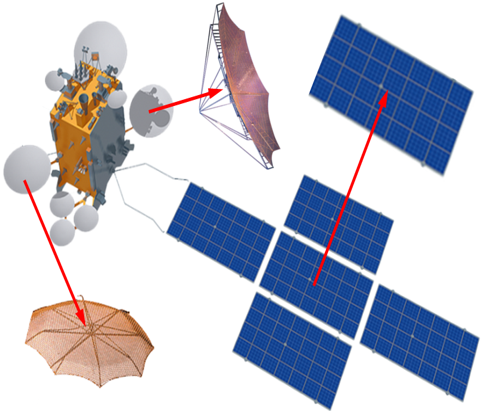
\includegraphics[width = \textwidth]{decomposition}
	\end{subfigure}
	\hfill
	\begin{subfigure}[b]{0.45\textwidth}
	     % Определение стиля
        \tikzstyle{blockWide} = [rectangle, draw = black, fill = blue!15, rounded corners, text width = 22em, text centered, minimum height = 1.5em, drop shadow] 
        \tikzstyle{blockWideC} = [blockWide, fill = red!20]
        \tikzstyle{arrow} = [draw, thick, color = black!90, -latex'] 
        \scriptsize 
        % Задание перменных
        \def\nodeDist{0.4cm}
        % Отрисовка блок-схемы
        \begin{tikzpicture}[scale = 1, transform shape]
            % Задание узлов		
            \node (modalTests) [blockWide] {Модальные испытания \\ составных частей конструкции};
            \node (modelUpdating) [blockWide, below = \nodeDist of modalTests] {Коррекция математических моделей составных частей \\ конструкции по результатам испытаний};
            \node (checkInfluence) [blockWide, below = \nodeDist of modelUpdating] {Освобождение математических моделей \\ составных частей конструкции};
            \node (buildRealModel) [blockWide, below = \nodeDist of checkInfluence] {Синтез математической модели полной \\ конструкции из её составных частей};
            \node (buildMathModel) [blockWide, below = \nodeDist of buildRealModel] {Определение динамических характеристик полной математической модели};
            % Соединение узлов
            \draw [arrow] (modalTests.south) -- (modelUpdating.north);
            \draw [arrow] (modelUpdating.south) -- (checkInfluence.north);
            \draw [arrow] (checkInfluence.south) -- (buildRealModel.north);
            \draw [arrow] (buildRealModel.south) -- (buildMathModel.north);
        \end{tikzpicture}
	\end{subfigure}
    \caption{Схема методики верификации крупногабаритных трансформируемых конструкций} \label{fig:schemeDecomposition}
\end{figure}

Продемонстрируем работу этого подхода на примере тестового космического аппарата из раздела~\ref{struct:perturbation}. Заметим, что низшие формы собственных колебаний, соответствующие упругим движениям конструкции, происходят с преимущественным деформированием панелей солнечный батарей, размещенных на орбитальном и командно-сервисном модулях. Поэтому, с целью исключения конструктивно подобных движений, упростим модель \figref{fig:spacecraft-full-mesh}, оставив только орбитальный модуль и связанные с ним солнечные батареи. Полученная конечно-элементная модель с числом степеней свободы $ 18714 $ приведена на рисунке~\ref{fig:spacecraft-test-mesh}.

\begin{figure}[!htb]
	\centering
	\includegraphics[width = 0.8\textwidth]{spacecraft-test-mesh}
	\caption{Упрощенная конечно-элементная модель тестового космического аппарата} \label{fig:spacecraft-test-mesh}
\end{figure}

Ключевым элементом корректности решения задачи синтеза является обеспечение наиболее полного описания жесткостных и массовых характеристик узлов сопряжения составных частей: орбитального модуля и панелей солнечных батарей. При детальном рассмотрении это требование оказывается противоречивым. С одной стороны, при жестком закреплении мест стыковки происходит безвозвратная потеря информации о стыковочных степенях свободы. С другой стороны, при проведении испытаний упруго-вывешенной конструкции как составной части, реализуются формы колебаний без существенного деформирования интерфейсных областей. Для снятия этого противоречия предлагается проводить модальные испытания составных частей с использованием вспомогательных устройств, обладающих известными жесткостными и инерционными характеристиками. В этом случае устройства, будучи прикрепленными к интерфейсам, обеспечивают их качественное описание. В предельном случае, когда жесткостные характеристики вспомогательного объекта равны нулю, это соответствует размещению массы. Причем чем больше масса, тем сильнее оказываются деформации в рассматриваемой области~---~более полно раскрываются жесткостные характеристики. После выполнения коррекции дополнительные устройства исключаются из расчетных моделей.

Кроме того, имея в виду достижение физической согласованности скорректированных моделей, предлагается использовать результаты нескольких экспериментов при различных условиях закрепления одной составной части. Так, в рассматриваемом примере, коррекция орбитального модуля производится по частотам свободных колебаний и частотам колебаний~\figref{fig:test-spacecraft-orbital-mode}, которые реализуется при прикреплении больших масс ($ \approx 30 $ \% от массы конструкции) к узлам стыковки. Расчетные модели панелей солнечных батарей вблизи мест стыковки дополняются невесомыми пластинами, свободные ребра которых закреплены жестко. Это позволяет проводить одновременную коррекцию по частотам как свободных, так и стесненных колебаний.

Примем в качестве целевых значений коррекции частоты собственных колебаний исходных моделей, сведенные в таблице~\ref{tab:targetTestSpacecraft}. Для имитации погрешностей моделирования, изменим модули упругости конструктивных элементов составных частей. Так, жесткость рамы панелей солнечных батарей, орбитального модуля и соединительных элементов была понижена на $ 10 $ \% в то время, как модуль упругости солнечных батарей повышен на $ 5 $ \%.

\def\sfSpacecraft{0.48\textwidth}

\begin{figure}[!htb]
	\centering
	\begin{subfigure}[t]{\sfSpacecraft}
		\centering
		\includegraphics[width = \textwidth]{test-spacecraft-orbital-mode-1}
		\caption{} 
	\end{subfigure}
	\hfill
	\begin{subfigure}[t]{\sfSpacecraft}
		\centering
		\includegraphics[width = \textwidth]{test-spacecraft-orbital-mode-2}
		\caption{} 
	\end{subfigure}	
	\begin{subfigure}[t]{\sfSpacecraft}
		\centering
		\includegraphics[width = \textwidth]{test-spacecraft-orbital-mode-3}
		\caption{} 
	\end{subfigure}	
	\hfill
	\begin{subfigure}[t]{\sfSpacecraft}
		\centering
		\includegraphics[width = \textwidth]{test-spacecraft-orbital-mode-4}
		\caption{} 
	\end{subfigure}	
	\caption{Первые четыре упругие формы колебаний орбитального модуля с прикрепленными к узлам стыковки массами~(а~--~г)} \label{fig:test-spacecraft-orbital-mode} 
\end{figure}

\begin{longtblr}[
	caption = {Целевые значения для коррекции составных частей космического аппарата}, 
	label = {tab:targetTestSpacecraft}
]{
	colspec = {|X[c, -1]|X[c]|X[c]|X[c]|X[c]|},
	width = \textwidth, 
	hlines
}
	\SetCell[r = 3]{c} № тона & \SetCell[c = 4]{c} Частоты собственных колебаний, Гц &&& \\
	& \SetCell[c = 2]{c} Орбитальный модуль &  & \SetCell[c = 2]{c} Панели солнечных батарей & \\
	& Свободный с прикрепленной массой & Свободный & Закрепленные & Свободные \\ \hline
	1 & \SetCell[r = 6]{c} \textbf{---} & \SetCell[r = 6]{c} \textbf{---} & 1.591 & \SetCell[r = 6]{c} \textbf{---} \\
	2 & & & 5.193 & \\
	3 & & & 6.841 & \\
	4 & & & 10.070 & \\
	5 & & & 22.028 & \\
	6 & & & 26.398 & \\
	7 & 8.221 & 15.721 & 42.179 & 11.810 \\
	8 & 8.477 & 15.721 & 42.613 & 13.770 \\
	9 & 8.660 & 21.300 & 46.050 & 29.339 \\
	10 & 8.863 & 21.303 & 58.393 & 33.784 \\
	11 & 9.095 & 24.132 & 67.767 & 42.796 \\
	12 & 10.598 & 24.498 & 68.897 & 51.135 \\
	13 & 10.600 & 24.498 & 85.064 & 58.768 \\
	14 & 11.178 & 31.483 & 88.711 & 61.625 \\
	15 & 15.730 & 31.483 & 93.117 & 72.682 \\
\end{longtblr}

Проведем коррекцию составных частей космического аппарата по девяти частотам собственных колебаний, используя одновременно данные двух экспериментов. После этого выполним ассемблирование скорректированных моделей. Полученные погрешности в частотах синтезированной модели сведены в таблице~\ref{tab:resultUpdatingTestSpacecraft}. Дополнительно к этим результатам отметим, что при коррекции составных частей только по данным одного виртуального эксперимента, максимальная погрешность в частотах синтезированной модели составила $ 6.34 $ \%. Такое значительное расхождение свидетельствует в пользу необходимости учета результатов нескольких испытаний при коррекции.

\begin{longtblr}[
	caption = {Результаты коррекции и ассемблирования составных частей тестовой модели космического аппарата}, 
	label = {tab:resultUpdatingTestSpacecraft}
]{
	colspec = {|X[c, -1]|X[c]|X[c]|X[c]|X[c]|},
	width = \textwidth, 
	hlines
}
	\SetCell[r = 3]{c} № тона & \SetCell[c = 4]{c} Погрешность в частотах собственных колебаний, \% &&& \\
	& \SetCell[r = 2]{c} Без коррекции & \SetCell[c = 3]{c} Коррекция по девяти частотам && \\
	& & Панелей & Модуля & Панелей и модуля \\ \hline
	7 & -4.689 & -2.120 & -2.756 & -0.021 \\
	8 & -4.678 & -2.078 & -2.782 & -0.018 \\
	9 & -5.121 & -4.447 & -0.674 & 0.100  \\
	10 & -5.040 & -4.760 & -0.354 & -0.028 \\
	11 & -5.040 & -4.760 & -0.357 & -0.032 \\
	12 & -5.121 & -4.443 & -0.687 & 0.091 \\
	13 & -4.102 & -0.966 & -3.161 & 0.011 \\
	14 & -4.112 & -0.999 & -3.135 & 0.016 \\
	15 & -3.303 & -0.234 & -3.066 & -0.006 \\
	16 & -3.303 & -0.234 & -3.066 & -0.005 \\
\end{longtblr}

Распределение изменений узловых жесткостей по всем линейным степеням свободы для орбитального модуля и панелей солнечный батарей показано на рисунках~\ref{subfig:test-orbital-distribution}~и~\ref{subfig:test-panel-distribution} соответственно. При этом минимальный критерий модального соответствия, связывающий формы собственных колебаний синтезированной модели до и после коррекции, составил $ 0.9996 $.

Сходимость процедуры коррекции показана на рисунке~\ref{fig:test-spacecraft-convergence}. Она оценивалась посредством частотного критерия $ \lVert \mat{\alpha} \rVert_{\max} $:
\begin{equation}
	\alpha_{i, j} = \abs{1 - \frac{f ^ \ast_{i, j}}{f_{i, j}}}, \ i = 1 \hdots s, \ j = 1 \hdots r, \label{eq:convergenceCriterion}
\end{equation}
где $ s $~---~число корректируемых тонов колебаний, $ r $~---~число испытаний (моделей) для коррекции, $ f $ и $ f ^ \ast $~---~текущие и целевые значения частот. 

\begin{figure}[!htb]
	\centering
	\begin{subfigure}[t]{\sfSpacecraft}
		\centering
		\includegraphics[width = \textwidth]{test-spacecraft-orbital-distribution}
		\caption{Орбитальный модуль} \label{subfig:test-orbital-distribution} 
	\end{subfigure}
	\hfill
	\begin{subfigure}[t]{\sfSpacecraft}
		\centering
		\includegraphics[height = \textwidth]{test-spacecraft-panel-distribution}
		\caption{Панели солнечных батарей} \label{subfig:test-panel-distribution} 
	\end{subfigure} 
	\caption{Распределение изменений узловых жесткостей по всем линейным степеням свободы при коррекции составных частей по девяти тонам собственных колебаний} 
\end{figure}

\begin{figure}[!htb]
	\centering
	\includegraphics[width = 0.5\linewidth]{test-spacecraft-convergence}
	\caption{Сходимость частотного критерия при коррекции орбитального модуля и панелей солнечных батарей}  \label{fig:test-spacecraft-convergence}
\end{figure}

\section{Программная реализация методик коррекции, освобождения и синтеза}

\fixme{Предваряя следующую главу, нужно сказать о программной реализации: KLPCOR, KLPMRG, KLPEIG и KLPFREE. Краткое описание архитектуры. Более подробно об управляющих файлах для коррекции. Отметить универсальность комплекса при работе с разными КЭ-пакетами. Иллюстрация на примере PchConverter~---~Femap.}

\section{Выводы по главе \thechapter}